\documentclass[final]{fhnwreport}       %[mode] = draft or final
                                        %{class} = fhnwreport, article, 
                                        %          report, book, beamer, standalone
%%---Main Packages-----------------------------------------------------------------------
\usepackage[english, ngerman]{babel}	%Mul­tilin­gual sup­port for LaTeX
\usepackage[T1]{fontenc}				%Stan­dard pack­age for se­lect­ing font en­cod­ings
\usepackage[utf8]{inputenc}				%Ac­cept dif­fer­ent in­put en­cod­ings
\usepackage{lmodern}                    %The newer Font-Set
\usepackage{textcomp}				%LaTeX sup­port for the Text Com­pan­ion fonts
\usepackage{graphicx} 					%En­hanced sup­port for graph­ics
\usepackage{float}						%Im­proved in­ter­face for float­ing ob­jects
\usepackage{ifdraft}                    %Let you check if the doc is in draft mode


%%---Useful Packages---------------------------------------------------------------------
\usepackage[pdftex,dvipsnames]{xcolor}  %Driver-in­de­pen­dent color ex­ten­sions for LaTeX
\usepackage{csquotes}                   %Simpler quoting with \enquote{}
\usepackage{siunitx} 					%A com­pre­hen­sive (SI) units pack­age
\usepackage{listings}					%Type­set source code list­ings us­ing LaTeX
\usepackage[bottom]{footmisc}			%A range of foot­note op­tions
\usepackage{footnote}					%Im­prove on LaTeX's foot­note han­dling
\usepackage{verbatim}					%Reim­ple­men­ta­tion of and ex­ten­sions to LaTeX ver­ba­tim
\usepackage[textsize=footnotesize]{todonotes} %Mark­ing things to do in a LaTeX doc­u­ment

%%---Tikz Packages-----------------------------------------------------------------------
\usepackage{standalone}
\usepackage{tikz}
\usepackage{circuitikz}
\usetikzlibrary{arrows}
\usetikzlibrary{calc}
\usetikzlibrary{intersections}

%%---Math Packages-----------------------------------------------------------------------
\usepackage{amsmath}					%AMS math­e­mat­i­cal fa­cil­i­ties for LaTeX
%\usepackage{amssymb}					%Type­set­ting symbols (AMS style)
%\usepackage{array}						%Ex­tend­ing the ar­ray and tab­u­lar en­vi­ron­ments
%\usepackage{amsthm}					%Type­set­ting the­o­rems (AMS style)

%%---Table Packages----------------------------------------------------------------------
\usepackage{tabularx}					%Tab­u­lars with ad­justable-width columns
%\usepackage{longtable}
\usepackage{multirow}					%Create tab­u­lar cells span­ning mul­ti­ple rows
\usepackage{multicol}					%In­ter­mix sin­gle and mul­ti­ple columns

%%---PDF / Figure Packages---------------------------------------------------------------
\usepackage{pdfpages}					%In­clude PDF doc­u­ments in LaTeX
\usepackage{pdflscape}					%Make land­scape pages dis­play as land­scape
\usepackage{subfig}					    %Fig­ures di­vided into sub­fig­ures

%%---Other Packages----------------------------------------------------------------------
%\usepackage{xargs}                     %De­fine com­mands with many op­tional ar­gu­ments

%%---Bibliography------------------------------------------------------------------------
\usepackage[style=ieee,urldate=comp,backend=biber]{biblatex}
\addbibresource{literature/bibliography.bib}

%%---Main Settings-----------------------------------------------------------------------
\graphicspath{{./graphics/}}			%Defines the graphicspath
%\geometry{twoside=false}				    %twoside=false disables the "bookstyle"
\setlength{\marginparwidth}{2cm}
\overfullrule=5em						%Creates a black rule if text goes over the margins => debugging


%%---User Definitions--------------------------------------------------------------------
%%Tabel-Definitions: (requires \usepackage{tabularx})
\newcolumntype{L}[1]{>{\raggedright\arraybackslash}p{#1}}    %column-width and alignment
\newcolumntype{C}[1]{>{\centering\arraybackslash}p{#1}}
\newcolumntype{R}[1]{>{\raggedleft\arraybackslash}p{#1}}




%%---Optional Package Settings-----------------------------------------------------------
%Listings-Settings: (requires \usepackage{listings}) => Example with Matlab Code
\lstset{language=Matlab,%
    basicstyle=\footnotesize\ttfamily,
    breaklines=false,%
    morekeywords={switch, case, otherwise},
    keywordstyle=\color{Blue},%
    tabsize=2,
    %morekeywords=[2]{1}, keywordstyle=[2]{\color{black}},
    identifierstyle=\color{Black},%
    stringstyle=\color{Purple},
    commentstyle=\color{Green},%
    showstringspaces=false,%without this there will be a symbol in the places where there is a space
    numbers=left,%
    numberstyle={\tiny \color{black}},% size of the numbers
    numbersep=9pt, % this defines how far the numbers are from the text
    %emph=[1]{word1, word2,...},emphstyle=[1]\color{red}
}										                %loads all packages, definitions and settings												
\title{Elektrische Abroll- und Einzugswinde}          %Project Title
\author{Fachbericht}          %Document Type => Technical Report, ...
\date{Windisch, 13.08.2018}             %Place and Date

\begin{document}

%%---TITLEPAGE---------------------------------------------------------------------------
\selectlanguage{ngerman}                %ngerman or english
\maketitle

\vspace*{-1cm}						    %compensates the space after the date line.
\vfill
\begin{figure}[H]
\centering

\includegraphics[width=\linewidth]{titelbild.pdf}
\end{figure}
\vfill

{
\renewcommand\arraystretch{2}
\begin{center}
\begin{tabular}{>{\bf}p{4cm} l}
Hochschule                 &    Hochschule für Technik - FHNW\\
Studiengang                &    Elektro- und Informationstechnik\\
Autor   		           & 	Philipp Duthaler und Severin Hunziker\\
Betreuer                   &    Felix Jenni\\
Auftraggeber               &    Daniel Egli\\
Version                    &    1.0 %Normally not used!
\end{tabular}
\end{center}
}

\clearpage
			
%%---ABSTRACT----------------------------------------------------------------------------
\selectlanguage{ngerman}				%ngerman or english
\thispagestyle{empty}
\begin{abstract}
For a long time, not only the weather but also the terrain determined whether a paraglider could be flown. Towing winches can practically eliminate the terrain factor, but in order to cover all eventualities, both pull-in winches and roll-off winches still have to be purchased as separate systems. To solve this problem, the DualModeWinch is being developed in this project. It has both the pull-in winch and the roll-off winch in one system. It is the first winch on the market that combines both functions in one device. This is made possible by the installation of an electric motor which can be operated both in forward and reverse direction. In addition, the power supply is provided by batteries which when compared to conventional towing winches enables low-noise, no C02 emissions and an energy-efficient operation. The motor is monitored by a controller during the towing process. It also ensures that the operation is as error-free and safe as possible. The DualModeWinch is delivered as a complete package and can be transported in a car with boot size of 90x60x90cm. It is therefore suitable for private individuals as well as for larger paragliding clubs. The central elements of the winch are the motor and the associated controller, whereby the controller regulates the motor in both operating modes. The first performance tests in pull-in winch operation were successful. All legal requirements for the winch as well as all possible operating conditions for torque and speed were achieved. In a future step, all important components for the discharge circuit, the heating resistor and the batteries must be determined, ordered and assembled for the test setup. In summary, it can be said that all general conditions and legal requirements have been met and a large part of the functionality of the winch could be tested.


\vspace{2ex}
\textbf{Keywords: Dual mode, Electric, Paraglide, Winch}
\end{abstract}	





%%---TABLE OF CONTENTS-------------------------------------------------------------------
\pagenumbering{Roman}		
\selectlanguage{ngerman}				%ngerman or english
\tableofcontents
\clearpage

%%---TEXT--------------------------------------------------------------------------------
\pagenumbering{arabic}
\section{Einleitung}
Vor über 50 Jahren stürzten sich mit den ersten Gleitschirmen waghalsige den Hang herunter. Die Technologie machte wahnsinnige Fortschritte, jedoch blieb das Startgelände lange den Bergen verwahrt. Obwohl die Schweiz über hohe Berge verfügt und dementsprechend viele Gleitschirmpiloten von Bergen her starten, gibt es gerade im nördlichen Teil der Schweiz, aufgrund von niedrigeren und bewaldeten Bergen, praktisch keine Startmöglichkeiten. Um dem entgegenzuwirken wurden sogenannte Abroll- und Einzugswinden entwickelt, welche einen Start in flachem Gelände ermöglichen. Da diese Technik bereits länger existiert, und die meisten Varianten auf einer Lösung mit Verbrennungsmotoren beruht, sind elektrisch betriebene Winden bisher kaum vertreten. Durch den technischen Fortschritt von Akkumulatoren ist ein regelrechter Aufschwung im Bereich von elektrischen Anwendungen im Gange. Mit der Kombination eines Elektromotors sind diverse Vorteile gegeben wir beispielsweise ein geräuscharmer Betrieb, keine CO2 Emissionen, einem hohen Wirkungsgrad und einer bidirektionalen Anwendung. Letzterer Punkt ermöglicht den Betrieb so wohl in Vorwärtsrichtung (als Motor), als auch in Rückwärtsrichtung (als Generator). Dies ermöglicht für den Abrollwinden-, und den Einzugswindenbetrieb die selbe Winde zu verwenden, was bis zum jetzigen Zeitpunkt absolut neuartig ist. Genau für diesen Zweck wird die Dualwinch entwickelt. Unser Ziel ist es, das Gleitschirmfliegen im Flachland zu revolutionieren und dabei die Umwelt nicht ausser Acht zu lassen. Dabei ist eine einfache und sichere Bedienung für jedermann und einem effektiven Schleppvorgang unsere Motivation.


\section{Grundlagen}\label{sec:Grundlagen}
In diesem Kapitel wird der grundlegende Ablauf des Schleppvorgang beschrieben und die Funktion der beiden Windentypen (Einzug- und Abrollwinde) genauer erklärt. Weiter sind die für dieses Projekt grundlegenden Anforderungen aufgelistet, wobei eine detaillierte Übersicht im Anhang \ref{appsec:Anforderungen} ersichtlich ist.

%für den Bericht grundlegende Informationen beschrieben. Diese werden zum einen in Richtlinien unterteilt,welche hauptsächlich aus den gesetzlichen Bestimmungen bestehen. Zum anderen ist ein mathematischer Teil vorhanden, wobei die Berechnungen mathematische Formeln aufweisen auf welche in den nachfolgenden Kapiteln verwiesen wird. 


\subsection{Schleppvorgang}\label{subsec:Schleppvorgang}
Der Gleitsegelschleppvorgang kann trotz zwei unterschiedlichen Ausführungen (Einzug- und Abrollwinde) mit demselben Prinzip beschrieben werden. Der Pilot steht startbereit am Boden und ist über auslösbare Verbindungen an ein Seil angemacht. Sobald der Schleppvorgang startet, wird das Seil zwischen Winde und Pilot gestraft bis er eine Kraft in horizontaler Richtung erfährt. Er beginnt zu rennen, wobei sich der Schirm über ihm aufrichtet. Sobald der Pilot eine genügend hohe Geschwindigkeit in Horizontalrichtung hat (in Bezug zum Wind), erfährt er eine Geschwindigkeit in Vertikalrichtung und hebt ab. Die dafür notwendige horizontal Geschwindigkeit ist abhängig vom Schirmtyp. Ein typischer Startvorgang ist in nachfolgender Abbildung \ref{fig:Sicherheitsstart} gut ersichtlich. Es gilt zu erwähnen, dass der ersichtliche Schleppvorgang bei einem Gegenwind von 5m/s abgebildet ist. Bei einer Vorwärtsgeschwindigkeit von 5m/s erreicht somit der Pilot eine Horizontalgeschwindigkeit von 10m/s gegenüber Wind.

\begin{figure}[H]
	\begin{center}
		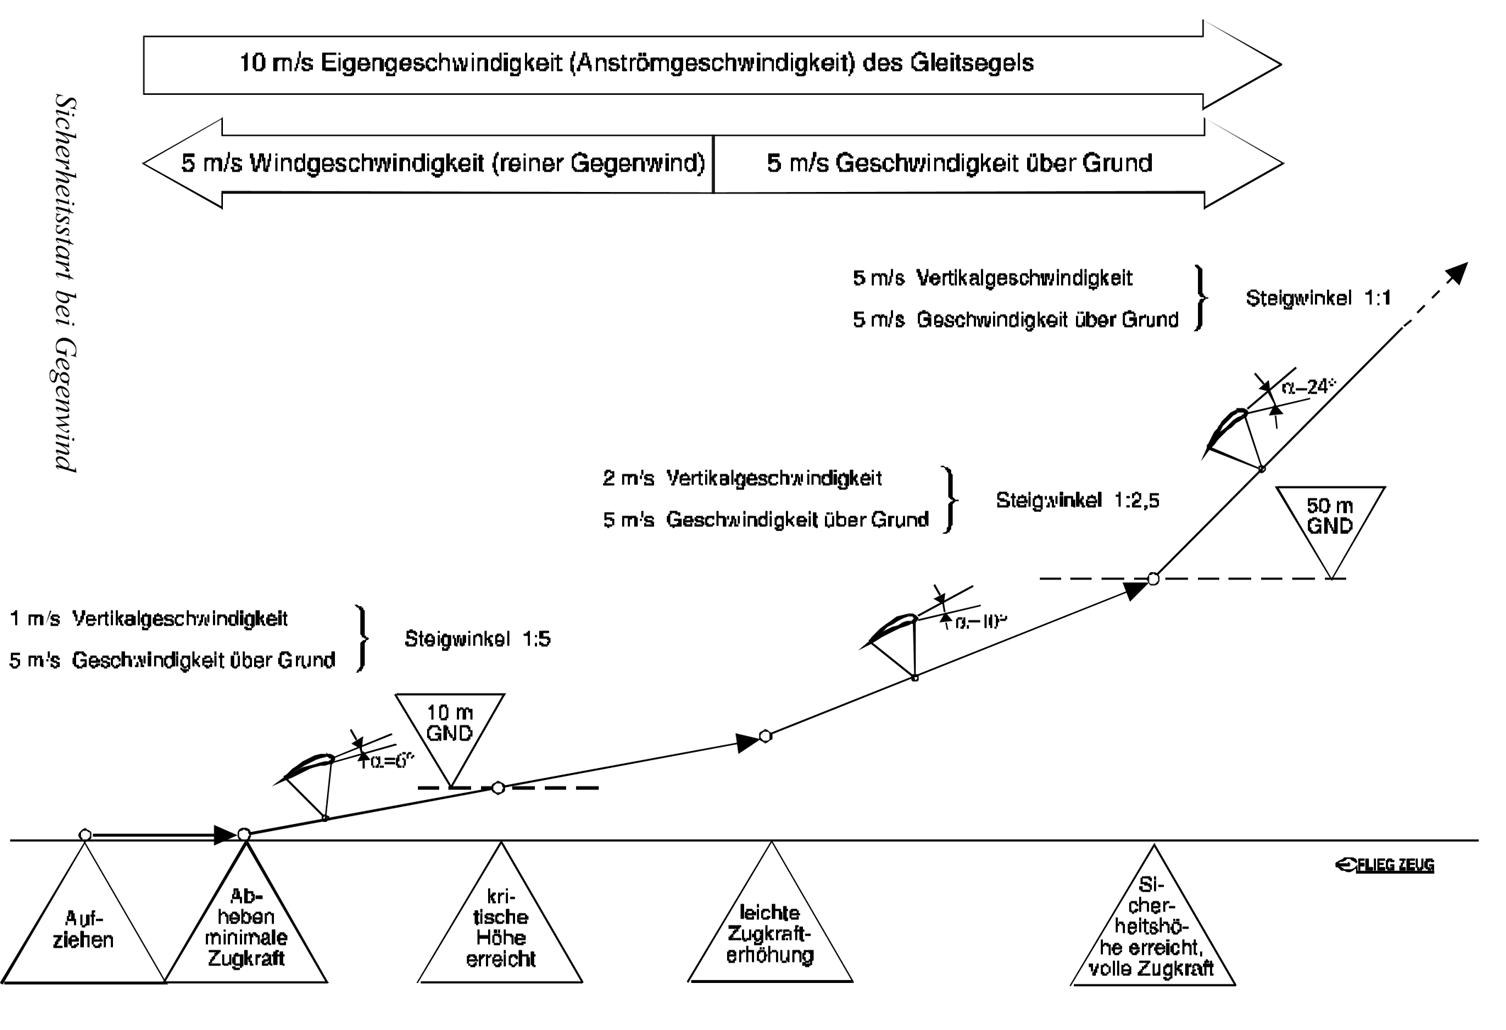
\includegraphics[width=160mm]{Sicherheitsstart.png}
		\caption{Sicherheitsstart beim Schleppvorgang \cite{Gleitsegelschlepp}}
		\label{fig:Sicherheitsstart}
	\end{center}
\end{figure}

In Abbildung \ref{fig:Sicherheitsstart} ist gut ersichtlich, dass der Startvorgang in vier Bereiche unterteilt wird. Die erste Phase beinhaltet die Seilstraffung bis zum Zeitpunkt des Abheben des Piloten. Der zweite Bereich umfasst die kritischste Phase, da der Pilot nur eine geringe Distanz zum Boden vorweist und bei einem Trennvorgang schnell reagieren muss. Damit ein unvorhergesehener Trennvorgang vom Piloten kontrolliert werden kann, darf die Zugkraft am Seil lediglich 30\% der Nennzugkraft betragen. Die Nennzugkraft wiederum ist vom Gewicht des Gleitschirmpiloten abhängig. Sobald eine Höhe von 20m erreicht wurde, wird der Zugkraft am Seil auf 70\% der eingestellten Nennzugkraft erhöht. Ab einer Höhe von 50m darf mit der vollen Nennzugkraft gezogen werden, wodurch der Pilot mit einem Winkel (gegenüber Grund) von rund $27^\circ$ steigt. Diese Phase hält solange an, bis der Pilot die gewünschte Höhe erreicht hat oder mangels Seillänge der Vorgang beendet werden muss. Die Zugkraft wird erneut reduziert, so dass die Zugkraft am Piloten abnimmt und der Schirm sich wieder über den Piloten neigt. Bei einer Zugkraft von wiederum 30\% der Nennzugkraft trennt sich nach Zeichenabsprache mit dem Windenführer der Pilot vom Seil. Diese Flugkurve mit den entsprechenden Steigwinkeln des Piloten gegenüber Grund ($\beta$) und dem Einzugswinkel des Seils ($\gamma$) ist in nachfolgender Abbildung \ref{fig:HoehenverlaufSchlepp} ersichtlich. Es gilt zu beachten, dass der Winkel $\gamma$ den Wert von 70° nicht überschreiten darf.


\begin{figure}[H]
	\begin{center}
		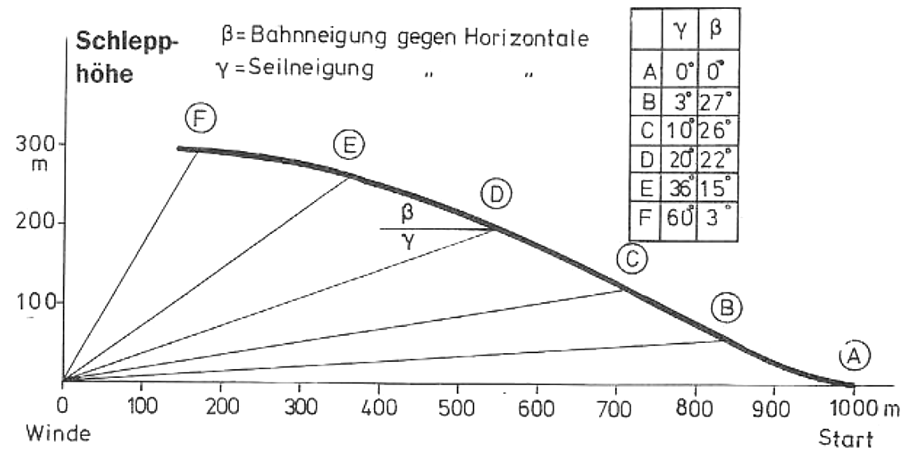
\includegraphics[width=120mm]{Windenstart.png}
		\caption{Höhenverlauf bei Schleppvorgang \cite{PhysikWindenschlepp}}
		\label{fig:HoehenverlaufSchlepp}
	\end{center}
\end{figure}

Es resultiert eine abgeflachte Kurve am Anfang und am Ende des Schleppvorganges. Sobald sich der Pilot vom Seil getrennt hat, wird das Seil durch einen bereits am Seil befestigten Fallschirm zu Boden geführt und auf der Winde eingezogen. Damit der nächste Pilot starten kann, müssen je nach Betriebsmodus unterschiedliche Massnahmen getroffen werden, deshalb werden nachfolgend der Einzugswinden- und Abrollwindenbetrieb genauer beschrieben.


\textbf{Einzugswindenbetrieb:}
Beim Einzugsbetrieb ist die Winde stationär am Boden befestigt und das Seil wird auf die gewünschte Länge ausgezogen. Bei Startbeginn befindet sich der Pilot gegenüber der Winde einige hundert Meter entfernt. Wird der Vorgang gestartet, so wird das Seil dementsprechend auf der Winde aufgerollt, respektive der Pilot zur Winde hingezogen. Die Einzugsgeschwindigkeit ist hierbei direkt von der Drehmoment Regelung abhängig und darf eine maximale Geschwindigkeit am Gleitschirm von 12m/s erreichen.

\textbf{Abrollwindenbetrieb:}
Beim Abrollwindenbetrieb wird die Winde an einem Auto (Ladefläche bei Pickup) befestigt. Das Auto übernimmt somit bei Betrieb die treibende Kraft und bewegt sich vom Piloten weg. Damit der Pilot, welcher beim Start lediglich einige Meter hinter dem Auto steht, eine Kraft in Horizontalrichtung erfährt und in die Luft gehoben wird, muss die Winde während dem Abrollvorgang bremsen. Die Kraftregulierung erfolgt direkt mit der Bremskraft mit welcher die Winde abgebremst wird. Die theoretisch maximale Kraft wird erreicht, wenn die Winde blockiert wird und sich somit der Pilot gleich schnell vorwärts bewegt wie das voreilende Fahrzeug. Es gilt zu beachten, dass die Bremsung elektrisch erreicht wird und dadurch der Elektromotor nicht exakt auf Drehzahl null herunter gebremst werden kann. Wie bereits in vorhergehenden Kapiteln erwähnt, hat ein Gleitschirm während dem Schleppvorgang gegenüber Luft eine Geschwindigkeit von 10m/s. Optimalerweise fährt der Fahrzeugführende mit einer Vorwärtsgeschwindigkeit, welche bei Windenblockade beim Piloten eine Vorwärtsgeschwindigkeit gegenüber Wind von 12m/s - 15m/s ergeben würde. Erfahrungsgemäss liegt in den meisten Fällen die Geschwindigkeit des Autos bei rund 50km/h.


\subsection{Anforderungen}\label{subsec:Richtlinien}
Die gesetzlichen Bestimmungen für die gesamte Seilwinde wurden bereits im Pflichtenheft thematisiert und aufgelistet. Nachfolgend werden daher lediglich die für die Auswahl von Motor und Controller, sowie dessen Validierung relevanten Vorschriften aufgeführt. Ausserdem sind auch Anforderungen an Energieversorgung und mechanischen Komponenten wie Seil und Sollbruchstellen kurz erläutert. Für eine detaillierte Erläuterung aller Anforderungen wird auf das technische Pflichtenheft \cite{TechPflichtenheft} verwiesen. Die Liste mit den Anforderungen aus dem Pflichtenheft sind zudem im Anhang \ref{appsec:Anforderungen} hinterlegt.

Durch die elektrische Versorgung des Motors, unterliegt das Projekt der Norm der IEC (International Electrotechnical Commission). Damit die Richtlinien möglichst tief gehalten werden können, fiel der Entschied auf den Kleinspannungsbereich (Spannungsbereich \RM{1} nach IEC 60449), was einer Spannung $U_{DC}<120V_{DC}$ oder $U_{AC}<50V_{AC}$ entspricht. Dies bringt den Vorteil mit sich, dass keine für den Mensch gefährlichen Spannungen auftreten können, was geringere Vorschriften an Isolation, Berührungsschutz und Leitungsführung mit sich bringt.
Die Anforderungen an den Betrieb der Winde gestalten sich durch nachfolgende Parameter. Die Zugkraft der Seilwinde (respektive des Seils) muss eine minimale Zugkraft von 600N erreichen und darf beim Einzelschlepp den Wert von $ 1000N $ nicht überschreiten. Werden zwei Personen gleichzeitig geschleppt (auch Doppelschlepp genannt), darf diese auf maximal $ 1300N $ erhöht werden. Die Zugkraft muss dem Windenführer stets bekannt sein und wird durch eine Kraftanzeige an einem Display erreicht.
Weiter darf während des Schleppvorgangs eine maximale Welligkeit von $\pm 25N$ auftreten. Das bedeutet, dass ein Oszillierender Einzug mit der genannten Kraftamplitude erlaubt ist. Wird der Winde ein Drehmoment-Sollwert vorgegeben, so darf diese nicht mehr als $\pm 100N$ davon abweichen. Das bedeutet, bei maximaler Zugkraft (im Einzelschlepp) dürfen Werte zwischen $ 900N $ und $ 1100N $ auftreten. Aus Sicherheitsgründen wird die maximale Einzugsgeschwindigkeit begrenzt. Da bei Nullwind eine Einzugsgeschwindigkeit von 10m/s für optimales Steigen sorgt und evt. leichte Rückenwinde während dem Schleppvorgang auftreten können, wurde die Geschwindigkeit des Seil auf maximal $ 12m/s $ gelegt.
Zur Sicherheit des Piloten, muss ein Schleppvorgang jederzeit abgebrochen werden können. Dies kann einerseits durch Leerlauf des Motors oder im schlimmsten Fall durch einen Kappvorgang des Seils erreicht werden. Neben der Kappvorrichtung müssen auch Vorseil, Schleppseil, Verbindungsteile und Reparaturstellen eine minimale Reissfestigkeit von > 4000N erreichen, so wie Sollbruchstellen mit einer Bruchlast von min. 1500N im Einzelschlepp und min. 2000N im Doppelschlepp \cite{WindenPruefanweisung}.


Da der Motor primär von Batterien gespiesen wird und diese eine begrenzte Kapazität vorweisen, wurde ein batteriebetriebener Schleppvorgang von minimal fünf Startvorgänge definiert. Ein weiterer Betrieb wird durch einen Hilfsgenerator ermöglicht, welcher lediglich zur Unterstützung der Batterie dient und somit nicht die gesamte Leistung übernimmt. Die Batterien müssen zudem sowohl gegen Tiefen- als auch gegen Überladung geschützt werden.
\section{Hardware}\label{sec:Hardware}
In diesem Kapitel werden die für den elektrischen Teil notwendigen Hardware Komponenten detailliert beschrieben. Dabei umfasst es jegliche Komponenten welche beim Betrieb einen elektrischen Anschluss besitzen wie beispielsweise Motor, Controller und die gesamte Energieversorgung. Da noch nicht alle Elemente bestimmt und ausgearbeitet wurden, fehlen einige Komponenten wie beispielsweise die Bremsschaltung mit entsprechendem Bremswiderstand oder evt. für den Betrieb notwendige Sensoren. Aus diesem Grund wird in diesem Kapitel lediglich die Auswahl von Motor und Controller, sowie eine erste Übersicht der Energieversorgung erläutert. Es gilt zu beachten, dass für dieses Projekt 

\subsection{Motor und Controller}\label{subsec:MotorController}
Um einen Gleitschirmpiloten in die Luft zu heben, muss der Motor auch über ein grosses Drehmoment und genügend Leistung verfügen. Aus der Literatur Gleitsegelschlepp \cite{Gleitsegelschlepp} ist ersichtlich, dass der Gleitschirmpilot mit bis zu 10m/s gezogen wird. Aus den Richtlinien, welche der deutsche Gleitschirmverband erlassen hat, ist wiederum ersichtlich, dass mit einer Zugkraft von bis zu $ 1000N $ bei Solopiloten und $ 1300N $ bei Tandempiloten gezogen werden darf \cite{WindenProtokoll}. Daraus lässt sich die maximale Leistung, welche das System auf den Gleitschirmpiloten ausüben darf, ausrechnen \cite{Kuchling}:


\begin{equation}
\centering
	P_{Seil}=F \cdot \nu=1300N \cdot 10m/s=13kW
\label{eq:LeistungSeil}
\end{equation}

$ P_{Seil} $\quad 	Leistung des Seils     \\
$ F $\qquad  Zugkraft des Seils    \\
$ \nu $\qquad  Geschwindigkeit     \\

Da es sich um ein reales System handelt und deswegen im Motor, in Übertragung und Übersetzung Verluste auftreten, wird für die erste Handrechnung mit einem Gesamtwirkungsgrad des Systems von $80\%$ gerechnet.

\begin{equation}
\centering
	P_{Motor}=\frac{P_{Seil}}{\eta}=\frac{13kW}{0.8}=16.3kW
\label{eq:LeistungMotor}
\end{equation}

$ P_{Seil} $\quad 	Leistung des Seils     \\
$ P_{Motor} $  Leistung des Motors    \\
$ \eta $\qquad  Wirkungsgrad     \\

Da diese Leistung nicht über einen längeren Zeitraum geleistet werden muss, darf die Nennleistung des Motors leicht unter den 16.3kW liegen. Als Realisierungsmöglichkeiten standen somit lediglich Wechselstrommotoren mit Wechselrichter, DC-Motoren oder Brushless DC (auch BLDC) Motoren in Frage kommen. Eine Auswahl an Motoren mit deren Controller ist im Anhang \ref{appsec:Motoren} aufgelistet.
Damit die Schleppwinde auf dem Markt wettbewerbsfähig ist, muss es sowohl günstig sein, als auch alle elektrischen und mechanischen Anforderungen gänzlich erfüllen. Aufgrund des besten Preis-/ Leistungsverhältnissen und der hohen Nennleistung mit $ 13kW $, fiel der Entscheid gemeinsam mit dem Auftraggeber auf den BLDC Motor des Herstellers $ Goldenmotors $. Da dieser Motor in verschiedenen Betriebsspannungen ausgeführt wird ($ 48V $, $ 72V $ und $ 96V $), war aufgrund der Verlustleistung (welche sich durch den Strom im Quadrat berechnet), ein möglichst kleinerer Strom und somit eine hohe Spannung anstrebenswert. Da die Energieversorgung durch Bleiakkus realisiert wird und diese eine hohe Leerlaufspannung aufweisen (geladen 14.4V statt 12V pro Batterie), wird bei den notwendigen 96V eine Spannung von rund 116V erreicht, was nach wie vor im Kleinspannungsbereich liegt. Aus diesem Grund wurde das 96V Modell ausgewählt. Durch diesen Entscheid können sowohl beim Versuchsaufbau als auch bei der finalen Konstruktion kleinere Leiterquerschnitte gefahren werden, welches wiederum geringere Materialkosten zur Folge hat. Weiter konnte zwischen einem luftgekühlten und wassergekühlten Modell entschieden werden, wobei aufgrund des aufwändigen Aufbaus einer Wasserkühlung, der Entschied auf eine Luftkühlung fiel.  

Damit die Verlustleistung so klein wie möglich gehalten werden kann, ist es notwendig den Strom so tief wie möglich zu halten. Da dieser Motor in verschiedenen Betriebsspannungen ausgeführt wird ($ 48V $, $ 72V $ und $ 96V $), wurde die Variante mit der höchsten Spannung ausgewählt. 

\subsection{Energieversorgung}\label{subsec:Energieversorgung}

Damit die Einzugswinde betrieben werden kann, wird das gesamte System von einer Batterie gespiessen. Wie im vorhergehenden Abschnitt \ref{subsec:MotorController} beschrieben, wurde ein Motor mit 96V Nennspannung ausgewählt. Aus diesem Grund ist es notwendig, Batterien mit derselben Versorgungsspannung zu verwenden. Durch die fortlaufende Weiterentwicklung von Akkumulatoren, stellte sich die Frage nach dem Typ und der notwendigen Kapazität für den Betrieb. Trotz der steilen Entwicklungskurve von Li-Ionen Akkus, sind sie im Vergleich zu kommerziellen Blei-Akkus, komplizierter und heikler in der Handhabung (Ladeschaltung mit Zellenüberwachung notwendig) und vor allem teurer. Es muss jedoch berücksichtigt werden, dass auch bei Bleiakkus zwischen zwei Typen unterschieden wird. Zum einen werden oft Starterbatterien (hohe Anlaufströme, kurze Laufzeit) verwendet, und zum anderen zyklenfeste Bleiakkumulatoren (lange Laufzeit, ausgelegt für viele Lade-/ Entladevorgänge). Man kann sich wohl gut vorstellen, dass die zyklenfesten Modelle besser in den Versorgungsbetrieb unseres Projektes passen, jedoch muss bedenkt werden, dass sie durch die hohe Zyklenfestigkeit auch wesentlich teurer sind als die herkömmlichen Modelle.

Um einen Überblick zu erhalten, befinden sich im Anhang \ref{appsec:Batterie} zwei Tabellen mit einigen Modellen von jedem Typen. Diese werden jeweils in den elektrischen Klassifizierungen (Typ, Spannung, Kapazität), wie auch weiteren Merkmalen (wie Gewicht, Preis, Anzahl Starts) mit einander verglichen. Die Zyklenfesten Batterien wurden zusätzlich mit der vom Hersteller Angegebenen Zyklenfestigkeit und den jeweiligen Innenwiderständen ergänzt. Der Innenwiderstand wurde zusätzlich als wichtig betrachtet, da bei hohen Strömen (gemäss dem Ohmschen Gesetz) eine Spannung über den Batterien abfällt. Daher gilt: Umso grösser der Innenwiderstand, desto grösser die abfallende Spannung über den Batterien, wodurch eine kleinere Spannung an den Motor gelangt.
Damit man ein Gefühl für die Grössenordnung der jeweiligen Kapazitäten erhält, wurden die Anzahl möglichen Starts berechnet. Dafür wurden zuerst einige Annahmen getroffen.

\begin{table}[H]
	\centering
	\begin{tabular}{C{5cm} C{2.5cm} C{2cm}}
		\multicolumn{3}{c}{}\\
	{Beschreibung} & {Index} & {Wert} \\ \hline
	Zugkraft    &   $ F_{Zug} $    & $10 kN$   \\
	Geschwindigkeit    &   $ v $    & $10 m/s$   \\
	Startzeit    &   $ t $   & $120 s$   \\
	Gesamtwirkungsgrad    &  $ \eta_{tot} $    & $80\%$   \\
	Auslastung    &  $ \theta $   & $80\%$  \\
	Batterieausnutzung    &  $ \kappa $    & $60\%$   \\
	Gesamte Batteriekapazität   &   $ Q $    &   \\
	Gesamte Batteriespannung    &   $ U_{Bat,tot} $    &   \\
	Energie für Startvorgang    &   $ W_{Start} $    &   \\
	Gesamtenergie von Batterie   &   $ W_{Bat} $    &   \\
	Anzahl Starts    &   $ n $    &    \\	
	\end{tabular}
	\caption{Annahmen für Berechnung}
	\label{tab:BerechnungAnzahlStart}
\end{table}

\begin{equation}
\centering
	W_{Start}=\frac{F_{Zug}\cdot v \cdot t}{\eta_{tot}\cdot 3600}\cdot \theta
\label{eq:EnergieStart}
\end{equation}

\begin{equation}
\centering
	W_{Bat}=U_{Bat,tot}\cdot Q \cdot \kappa
\label{eq:EnergieBatterie}
\end{equation}

\begin{equation}
\centering
	n=\frac{W_{Start}}{W_{Bat}}
\label{eq:AnzahlStarts}
\end{equation}


Die Modelle mit dem besten Preis-Leistungsverhältnis wurden grün hervorgehoben. Diese entsprechen jedoch nicht unbedingt der günstigsten Variante. Augenfällig ist, dass der zyklenfeste Blei-Vlies Akku von Long nicht wesentlich teurer ist als einige Konkurrenzprodukte des Blei-Säure Akku Typs. Betrachtet man die nachfolgenden Abbildungen, so ist das Entladeverhalten bei unterschiedlichen Strömen in Abbildung \ref{fig:EntladeStrom} zu sehen, und das Entladeverhalten bei unterschiedlicher Entladung in Abbildung \ref{fig:EntladeKapazität} ersichtlich. Diese Messungen beziehen sich beide auf den bereits genannten Blei-Vlies Akku des Herstellers $Long$.


\begin{figure}[H]
	\centering
	\begin{minipage}[h]{.48\linewidth} % [b] => Ausrichtung an \caption
		\centering
		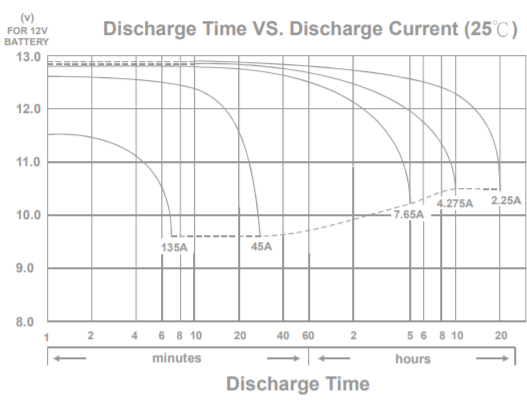
\includegraphics[width=\linewidth]{LongEntladeStrom.png}
		\caption[Batterie Entladeverhalten Strom]{Entladeverhalten Strom}
		\label{fig:EntladeStrom}
	\end{minipage}
	\quad % Abstand zwischen Bilder
	\begin{minipage}[h]{.48\linewidth} % [b] => Ausrichtung an \caption
		\centering
		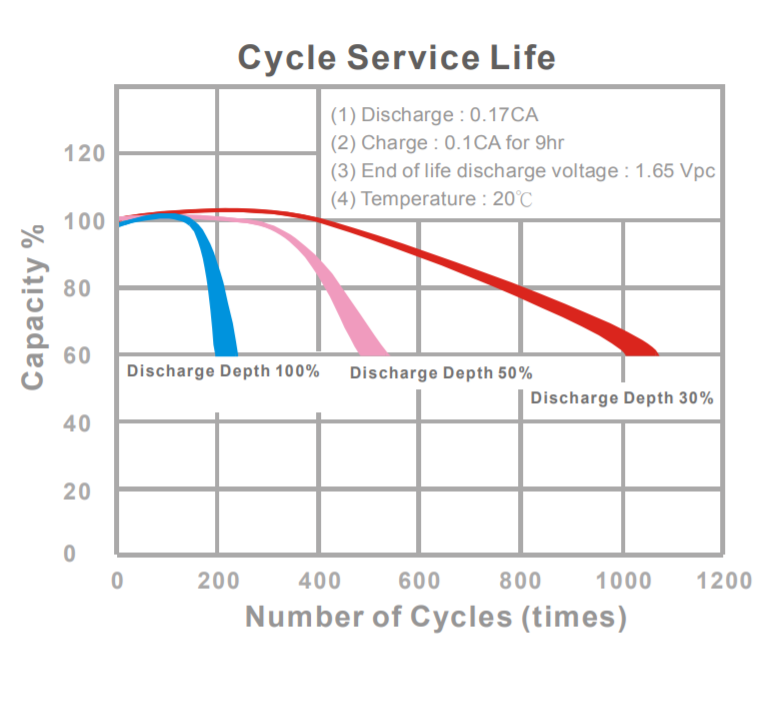
\includegraphics[width=\linewidth]{LongEntladeKapa.png}
		\caption[Batterie Entladeverhalten Kapazität]{Entladeverhalten Kapazität}
		\label{fig:EntladeKapazität}
	\end{minipage}
\end{figure}

In der linken Grafik ist unschwer zu erkennen, dass ab einer Spannung von rund 10.5V kaum Kapazität aus der Batterie herausgeholt werden kann und die Spannung stark abnimmt. Welche Auswirkung die Intensität eines Entladezyklus hat, ist in der rechten Abbildung ersichtlich. Wird die Batterie mit 100\% entladen, besitzt sie ab 200 Zyklen lediglich noch 60\% der Nennkapazität. Betrachtet man das kleine Kästchen innerhalb der \glqq Cycle\grqq Service Life Grafik, sind die Bedingen der Messung ersichtlich. Es gilt zu beachten dass die Temperatur beim Entladeversuch optimal auf 20°C gehalten wurden. Der Entlade-, sowie Ladestrom wird in den Datenblättern üblicherweise als CA Wert (Cranking Amperes) angegeben und ist eine Angabe welche sich auf die Kapazität der Batterie stützt. Der Strom berechnet sich gemäss nachfolgender Formel \ref{eq:CA}.

\begin{equation}
\centering
I=CA \cdot Q
\label{eq:CA}
\end{equation}
$ CA $\quad 	Cracking Amperes      \\
$ Q $\qquad  Kapazität Batterie     \\

Betrachtet man Abbildung \ref{fig:EntladeKapazität}, so ist ersichtlich dass der Strom bei der Entladung 7.65A und beim Ladevorgang 4.5A beträgt.
Wichtig ist der Wert der minimalen Zellenspannung welche 1.65V beträgt und auf keinen Fall unterschritten werden darf. Bei sechs Zellen resultiert eine minimale Spannung von 9.9V. Diese Berechnungen lassen sich auch auf andere Blei-Vlies Akkumulatoren übertragen und weichen meist nur wenig im Bereich der Zyklenfestigkeit und einem anderen CA-Wert ab.
\section{Software}
\section{Validierung}\label{sec:Validierung}
Das Ziel der Validierung ist es, abzuklären ob die gewählte Ansteuerung und der Brushless-Gleichstrommotor (BLDC) die verlangten Anforderungen erfüllen kann. Ausserdem wird das Steuerverhalten auf verschiedene Faktoren wie zum Beispiel Spannungsabfall, Laständerung und Steuerkennlinie untersucht.
Im ersten Unterkapitel wird die Versuchsanordnung erklärt mit welcher alle Versuche durchgeführt wird. Die darauffolgenden Unterkapitel beschreiben die jeweilige Messung und die Auswertung des Versuches.
Alle Messdaten sind im Anhang \ref{appsec:Messdaten} ersichtlich.


\subsection{Versuchsaufbau}\label{subsec:Versuchsaufbau}
Für den Versuchsaufbau wurde der BLDC mit einer asynchronen Maschine (ASM) gekoppelt, welche über einen Frequenzumrichter angesteuert wird und netzspeisefähig ist. Die ASM simuliert bei den nachfolgenden Versuchen die Last.


\begin{figure}[H]
	\begin{center}
		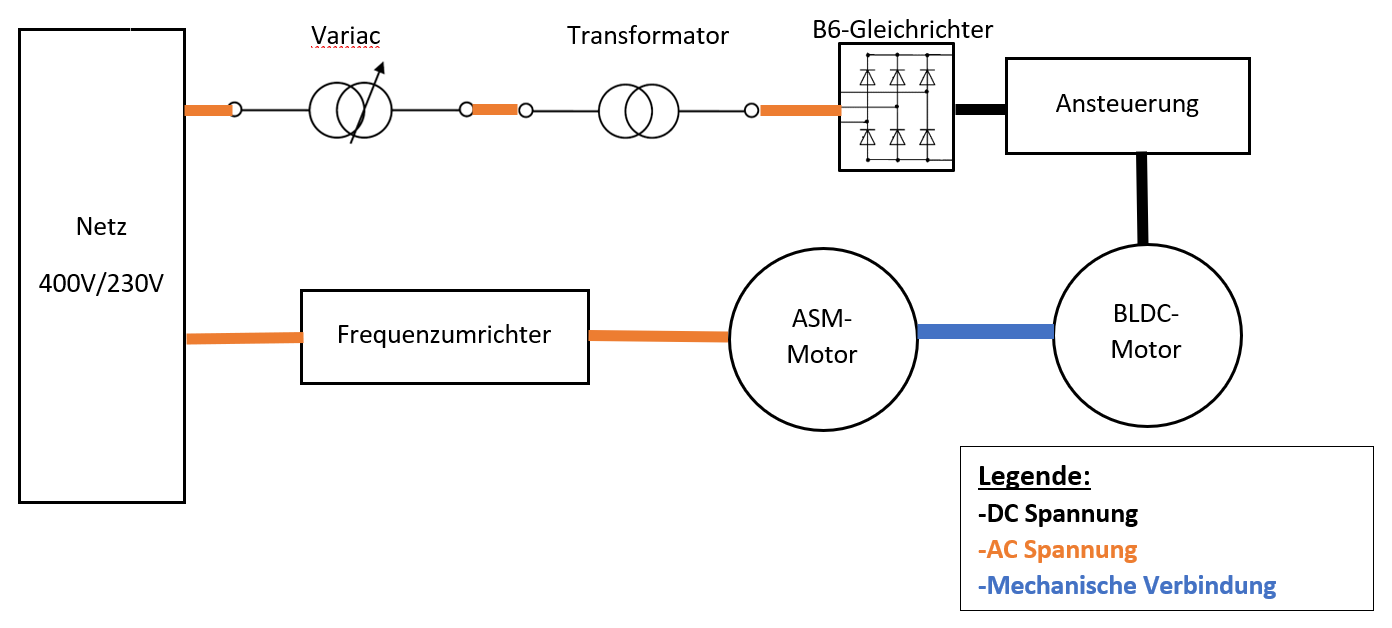
\includegraphics[height=70mm]{Versuchsaufbau/Schema.png}
		\caption{Schema Versuchsaufbau}
		\label{fig:Schema}
	\end{center}
\end{figure}

Um die verschiedene Versuche auszuwerten, wurde je nach Versuch verschiedene Gössen gemessen.
Die \textbf{Spannung} und der \textbf{Strom} wurde zwischen der Ansteuerung und dem B6-Gleichrichter gemessen. Die \textbf{Drehzahl} wurde mithilfe eines Oszillator ausgewertet. Dabei wurde dieser direkt an einem Hallsensor angehängt, welcher vier Impulse pro Umdrehung generiert. Die \textbf{Leistung} wurde mithilfe eines Power-Analyzers zwischen der ASM und dem Frequenzumrichter gemessen. Der \textbf{Drehmoment-Sollwert} wurde digital mit einem Mikrocontroller erzeugt und auf die Ansteuerung gegeben. Die \textbf{Motor-} und \textbf{Controller-Temperatur} wurden direkt am Computer ausgelesen, welcher an der Ansteuerung angeschlossen ist.\\

Wie auf dem Schema auf der Abbildung \ref{fig:Schema} ersichtlich, erfolgt die Energieversorgung durch das Netz und wird auf einen Variac (Abbildung \ref{fig:Variac}) geführt, welcher nachfolgend abgebildet ist.

\begin{figure}[H]
	\begin{center}
		\includegraphics[height=80mm]{Versuchsaufbau/DSC00555.jpg}
		\caption[Variac Versuchsaufbau]{Variac Versuchsaufbau}
		\label{fig:Variac}
	\end{center}
\end{figure}

Die Einspeisung des Variacs erfolgte durch eine CEE-63A Steckdose und ist auf der Abbildung nicht ersichtlich. Die Regulierung des Variacs erfolgt mittels drehen am kleinen schwarzen \glqq Steuerrad\grqq \space (unten links) und gibt bei Dreieckschaltung eine Ausgangsspannung zwischen 0-290V und einen maximalen Strom von 50A. Da unser Motor lediglich eine Betriebsspannung von 96V und im Nennbetrieb einen Strom von deutlich über 100A benötigt, wird ein Transformator nachgeschaltet (Abbildung \ref{fig:Trafo}). Der Anschluss erfolgte Primärseitig und Sekundärseitig in Dreieckschaltung und hat einen sekundären Maximalstrom von $95A_{AC}$ bei $127V_{AC}$. Die Gleichrichtung erfolgt mittels einer B6-Brücke, welche während diesem Projekt selber gebaut wurde. Der Aufbau ist in Abbildung \ref{fig:B6} ersichtlich.

\begin{figure}[H]
	\centering
	\begin{minipage}[H]{.4\linewidth} % [b] => Ausrichtung an \caption
		\centering
		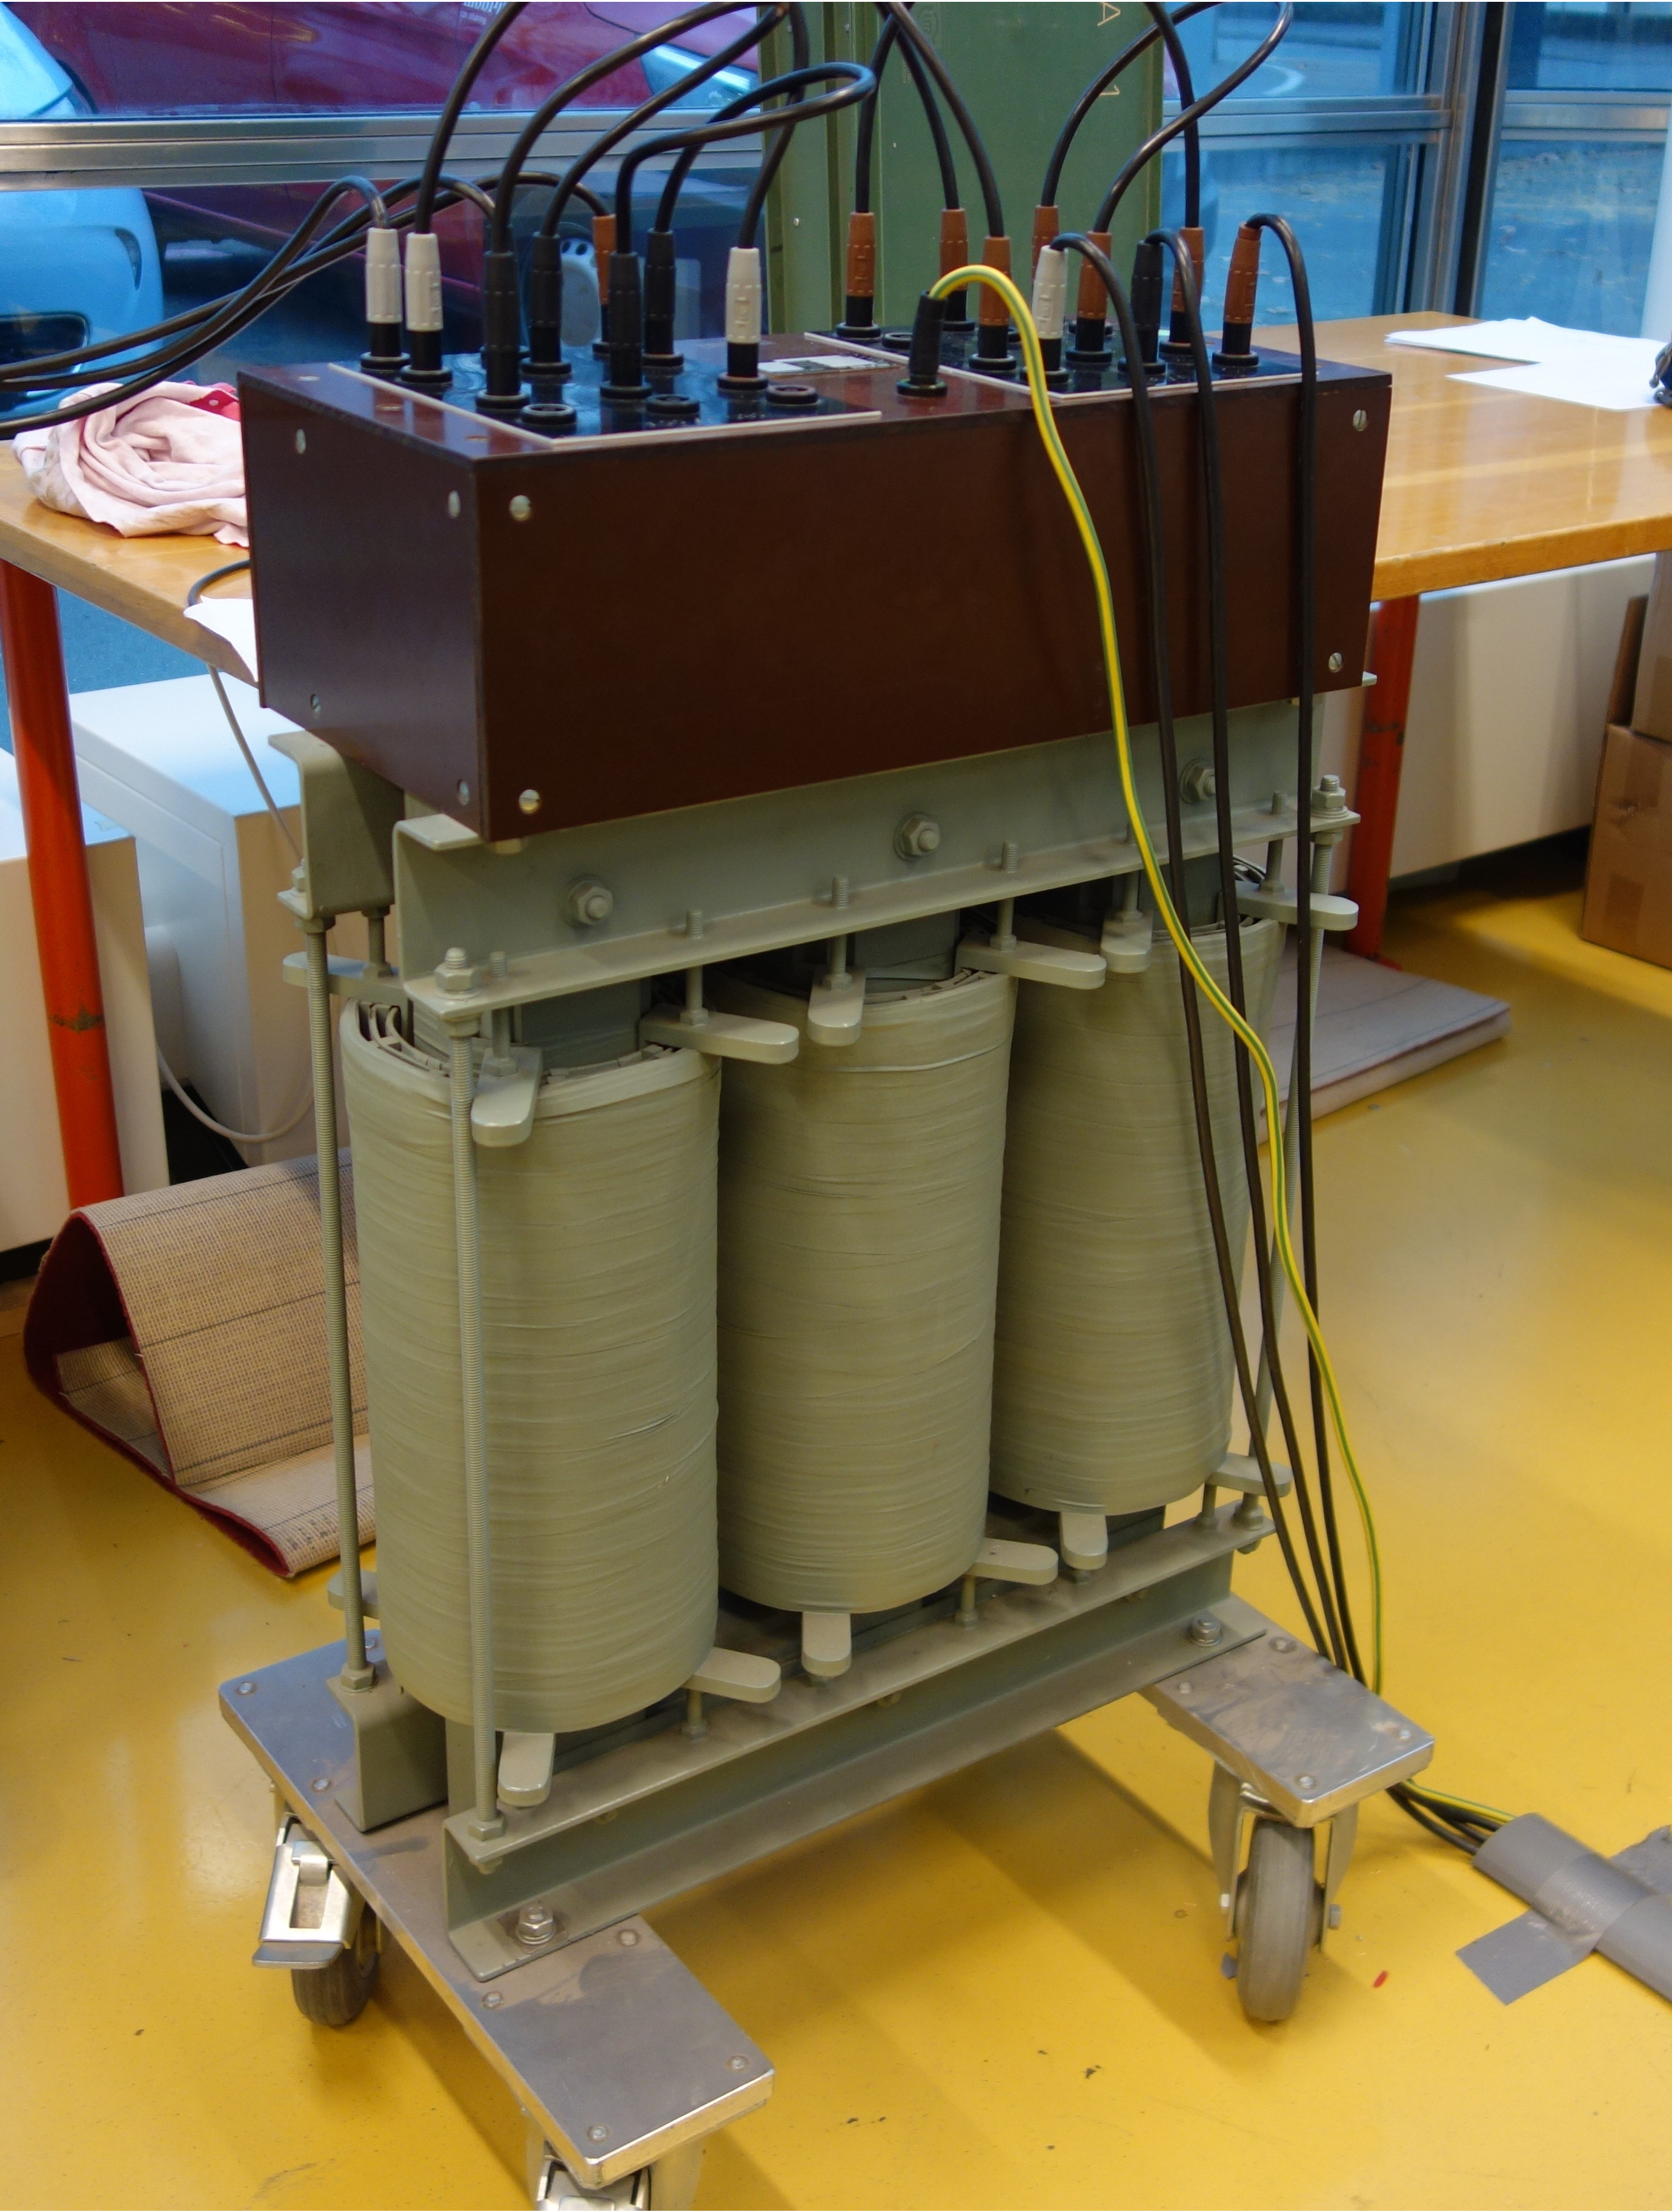
\includegraphics[width=\linewidth]{Versuchsaufbau/DSC00556.jpg}
		\caption[Transformator Versuchsaufbau]{Transformator}
		\label{fig:Trafo}
	\end{minipage}
	\ % Abstand zwischen Bilder
	\begin{minipage}[H]{.4\linewidth} % [b] => Ausrichtung an \caption
		\centering
		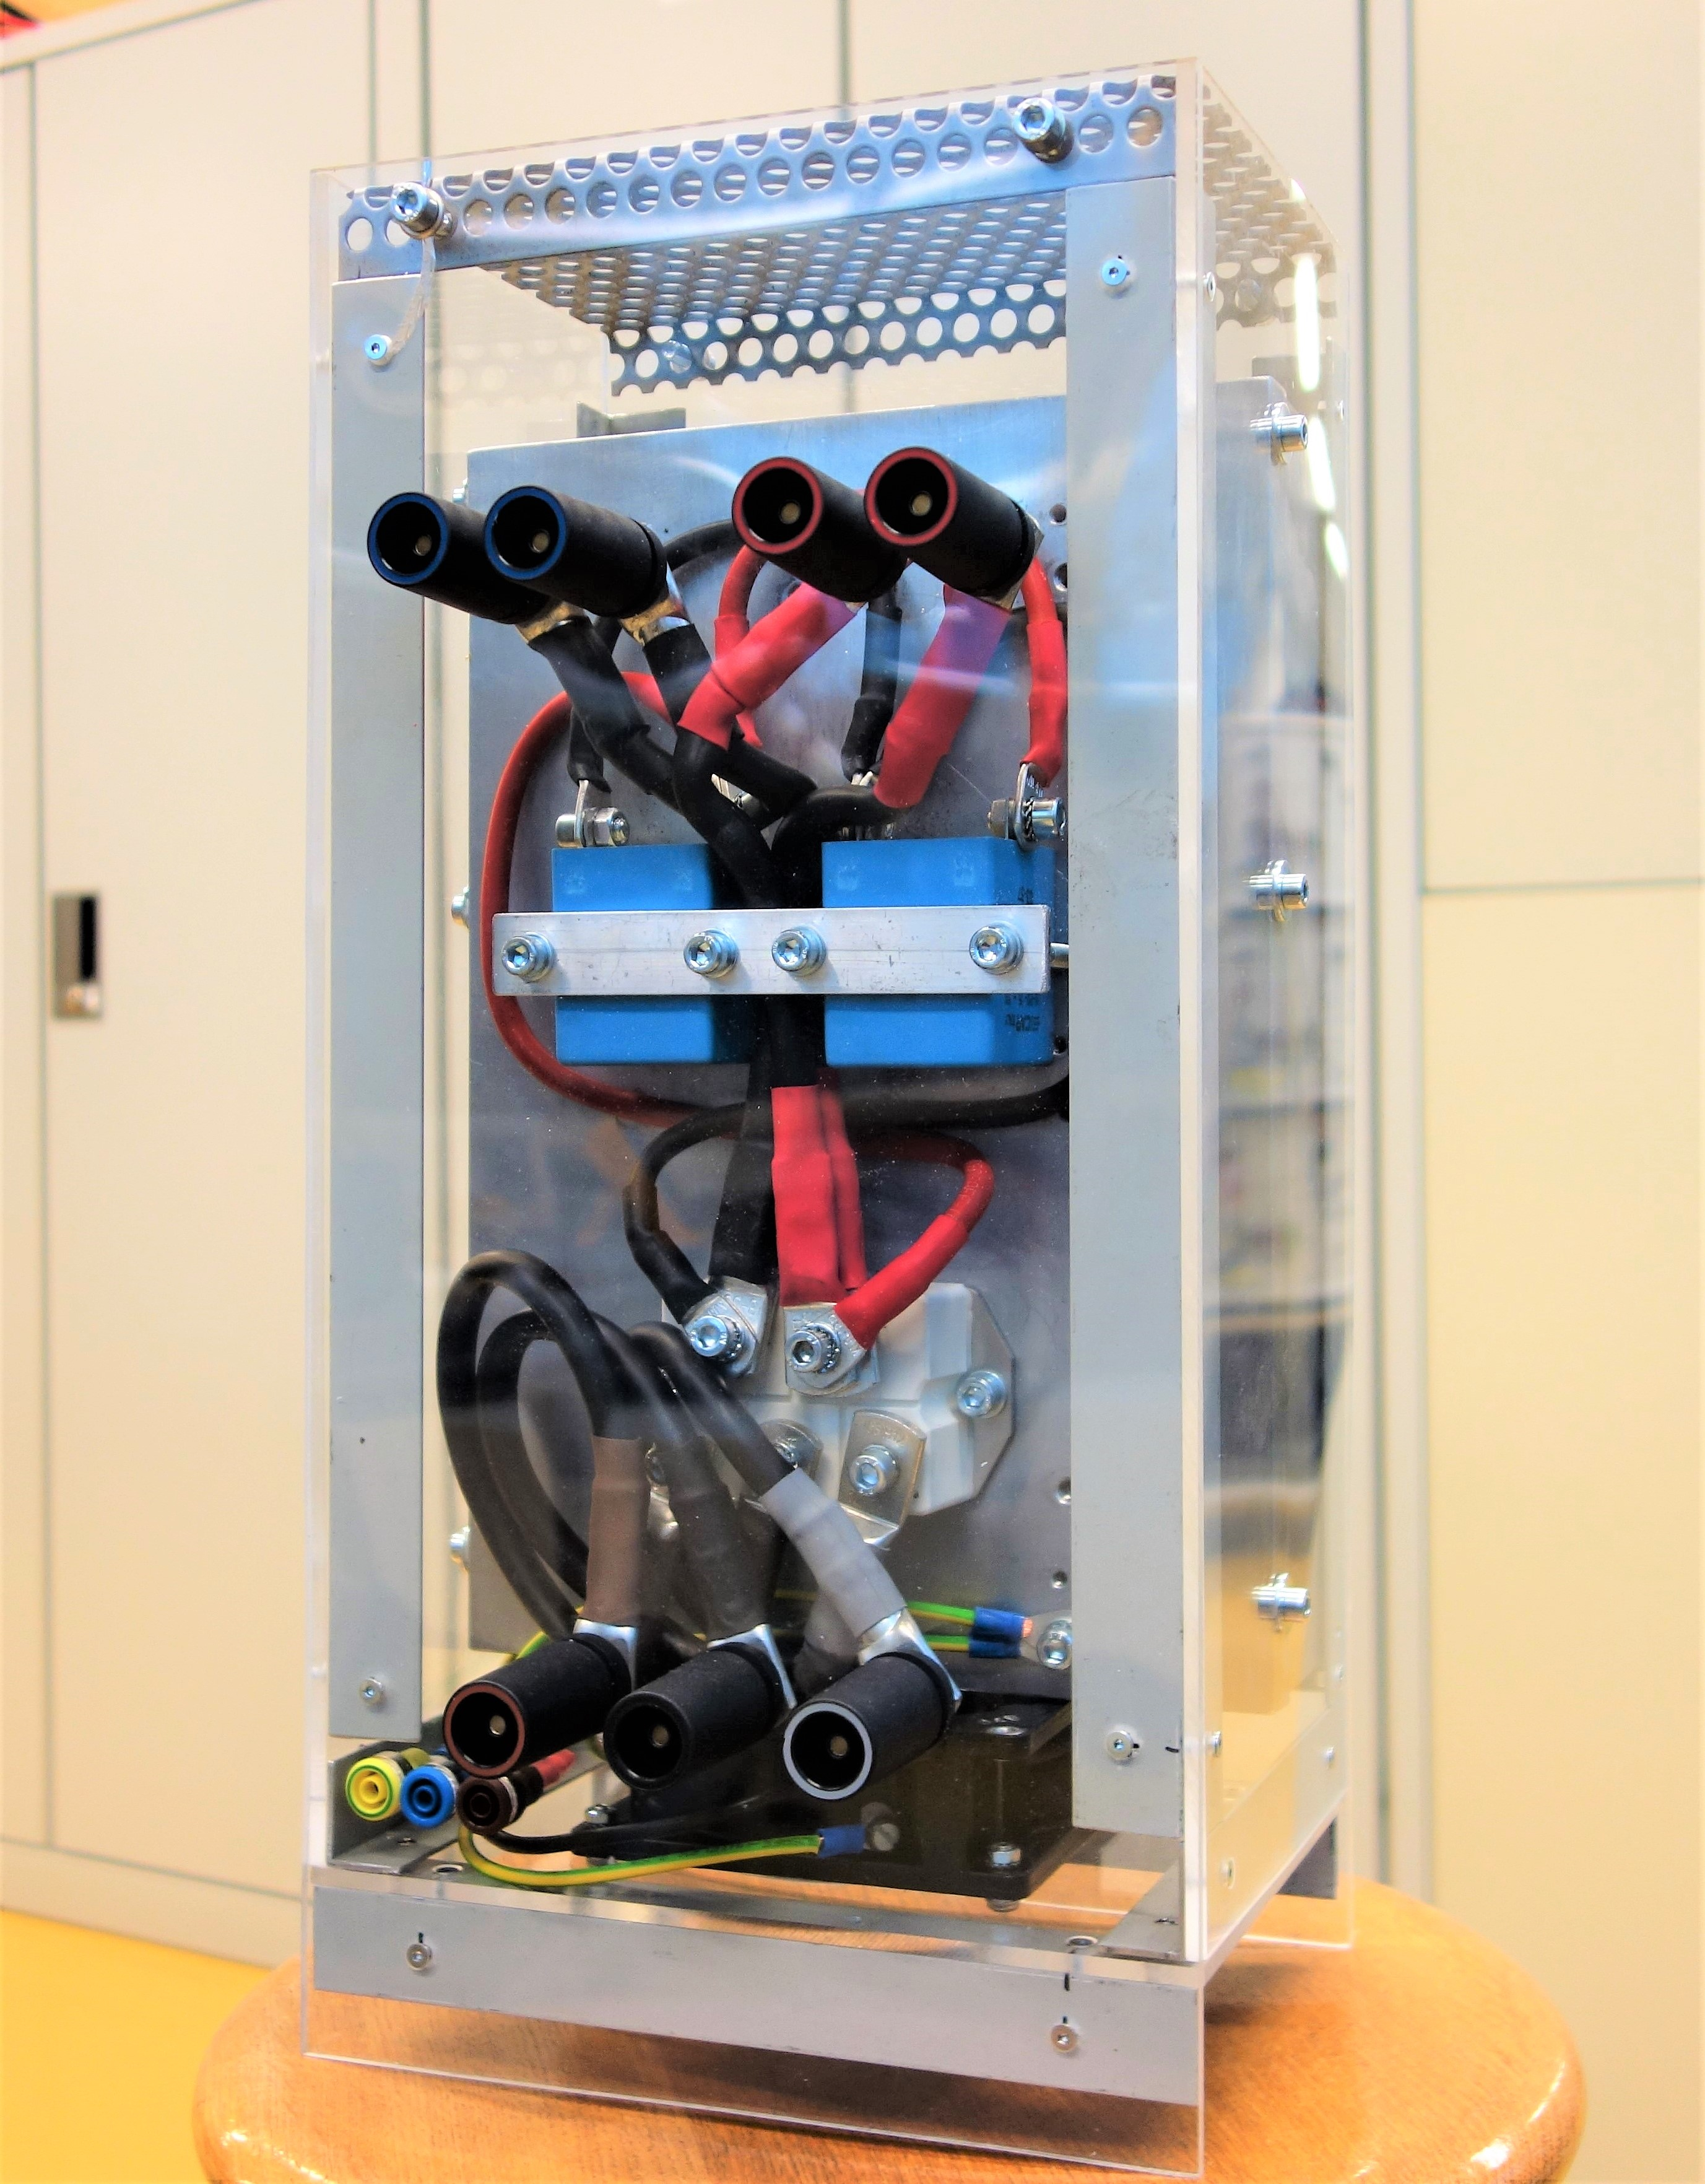
\includegraphics[width=\linewidth]{Versuchsaufbau/DSC00547(2).jpg}
		\caption[B6 Gleichrichter]{B6 Gleichrichter}
		\label{fig:B6}
	\end{minipage}
\end{figure}

Die AC-Einspeisung der B6-Brücke erfolgt mittels den drei Klemmen (Braun, Schwarz, Grau) im unteren Bereich. Diese werden auf den eigentlichen Diodengleichrichter (Weiss) und zwei Stützkondensatoren (Blau) geführt.Gemäss der Formel \ref{eq:B6-Id} ergibt sich somit einen maximalen Zwischenkreisstrom auf der DC Seite von $I_{DC}=\frac{95A}{0.8165} =\underline{116.35A}$.
Dieser erhöhte Strom, wird DC-Seitig durch jeweils zwei Hin-, und Rückleiter (Blau und Rot) auf die Motorenansteuerung geführt.\\
Die zwei Elektrolytkondensatoren (Elkos), welche in der Abbildung \ref{fig:Controller} ganz links ersichtlich sind, dienen zur Glättung der Gleichstromversorgung bei hohen Belastungen. Der Controller ist rechts im Bild ersichtlich, dazwischen befindet sich noch ein DC-Relais, welches vom Controller angesteuert wird und die DC-Speissung unterbrechen kann.

\begin{figure}[H]
	\begin{center}
		\includegraphics[height=80mm]{Versuchsaufbau/DSC00581.jpg}
		\caption[Controller]{Controller}
		\label{fig:Controller}
	\end{center}
\end{figure}

Tritt ein Fehlerfall auf, kann der Controller mithilfe des DC-Relais die Stromversorgung unterbrechen. Etwas schwer auf der Abbildung zu erkennen sind die Kontakte auf dem Controller. Dieser besitzt eine Sicherung direkt nach der Einspeisung des +Pols. Weiter ist ein geflechteter Kabelbaum ersichtlich (welcher alle Kabel zur Ansteuerung des Controllers beinhaltet) und die farbigen Anschlusskabel des Motors auf der rechten Seite.\\
Aus Sicherheitsgründen wurden alle blanken Elemente mit Klebestreifen isoliert und der Controller, die Elkos und das DC-Relais mit einer Kiste abgedeckt.

Der Drehmoment-Sollwert für die Ansteuerung wurde mit einem Arduino-Controller erzeugt. Dabei wurde der PWM-Ausgang mithilfe eines RC-Tiefpasses in ein Spannungssignal gewandelt. Mithilfe eines Schmitt-Triggers konnte zudem die Drehzahl des Motors gemessen und geregelt werden. Auf der Abbildung \ref{fig:Mikrocontroller} ist das Arduino-Board ersichtlich. Darauf aufgebaut ist eine Experimentierplatine mit drei Taster (rechts) um den Sollwert einzustellen, einem Schmitt-Trigger (mitte) und dem RC-Tiefpass (links).

\begin{figure}[H]
	\begin{center}
		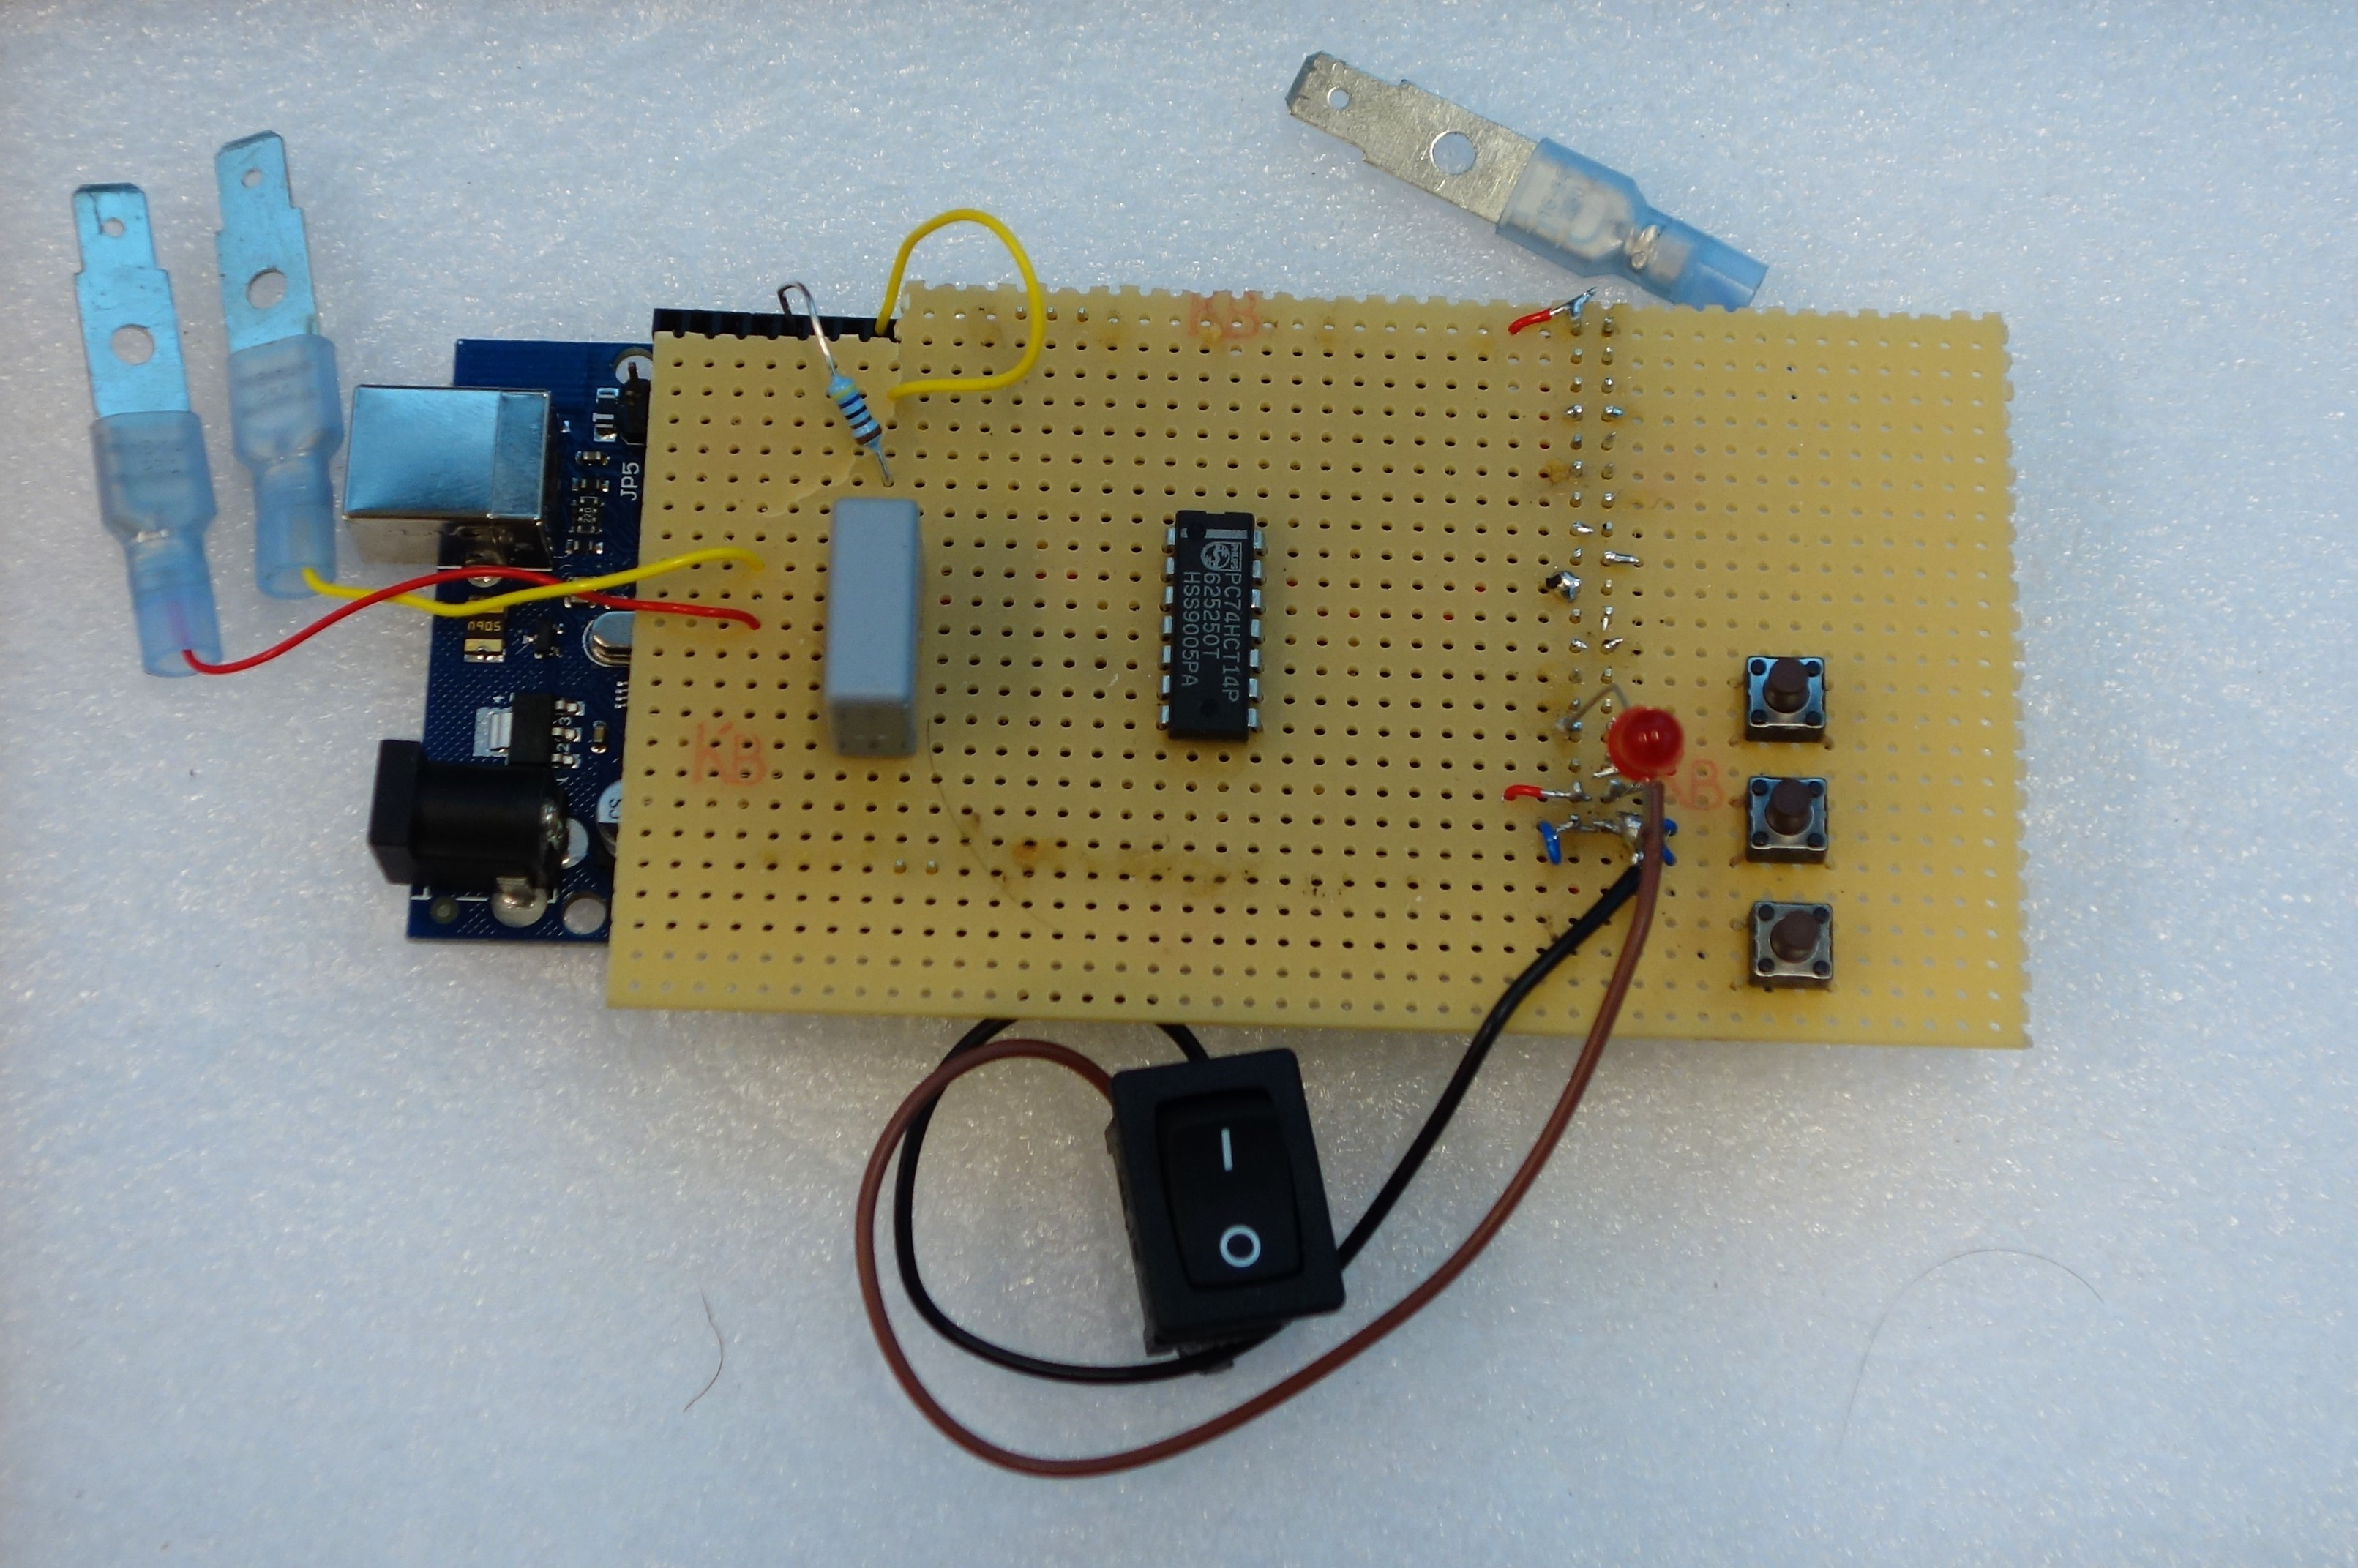
\includegraphics[height=60mm]{Versuchsaufbau/DSC00559.jpg}
		\caption[Controller]{Controller mit Experimentierplatine}
		\label{fig:Mikrocontroller}
	\end{center}
\end{figure}

Wie anfänglich bereits beschrieben wurde, wurde der verwendete BLDC Motor mit einer ASM gekoppelt. Die Anordnung ist in Abbildung \ref{fig:MotorenLueftung} links dargestellt. Damit diese zwei Maschinen überhaupt miteinander gekoppelt werden konnten, musste einerseits die Welle des BLDC Motors (links) auf das Niveau der ASM (rechts) angehoben werden und andererseits mussten einige Anpassungen an der Kupplung getätigt werden. Da der DC-Motor über eine Welle mit Zollmass verfügt, musste die Öffnung einer Kupplung ausgebohrt werden. Weiter verfügt die ASM über keine Nut, weshalb die andere Seite der Kupplung zur Befestigung mit einem Gewinde versehen werden musste. Die Befestigung erfolgt mittels zwei M8-Schraube, welche auf die Welle drücken. Für den Berührungsschutz sorgt eine Plexiglasscheibe über der mechanischen Verbindung.


\begin{figure}[H]
	\begin{center}
		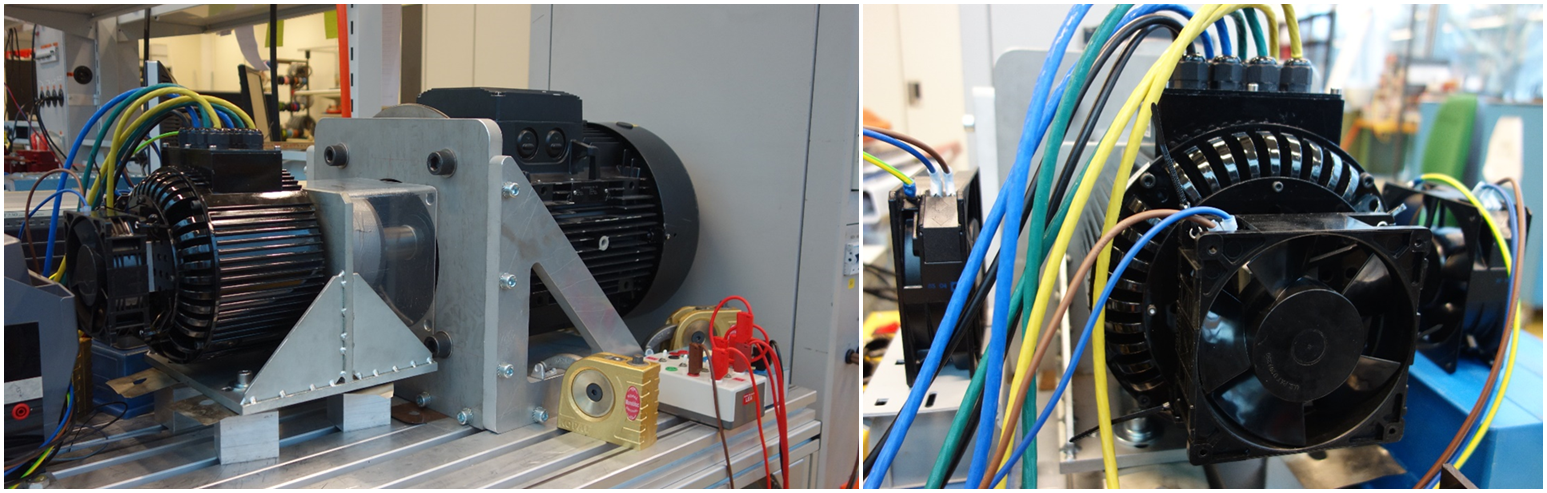
\includegraphics[width=\linewidth]{Versuchsaufbau/MotorLueft.png}
		\caption[Motoren Aufbau und Motorenlüftung]{Motoren Aufbau (links) und Motorenlüftung (rechts)}
		\label{fig:MotorenLueftung}
	\end{center}
\end{figure}

Leider weisst der verwendete Motor eine schlechte Eigenkühlung auf, wodurch zusätzliche Ventilatoren notwendig sind. In unseren Temperaturtests \ref{subsec:Temperatur} wurden zur Kühlung externe 110mm Ventilatoren verwendet. In Abbildung \ref{fig:MotorenLueftung} Grafik rechts, wurde die Anordnung seitlich und hinter dem Motor gewählt.


Damit überhaupt Leistungsversuche möglich sind, muss neben dem Gleichstrommotor auch die ASM angesteuert werden. Hierbei diente ein Frequenzumrichter (Abbildung \ref{fig:Frequenzumformer}) mit integrierter Netzschaltung. Die Versorgung erfolgt mittels einem CEE-32A Stecker und ist dementsprechend mit 32A abgesichert.

\begin{figure}[H]
	\centering
	\begin{minipage}[h]{.4\linewidth} % [b] => Ausrichtung an \caption
		\centering
		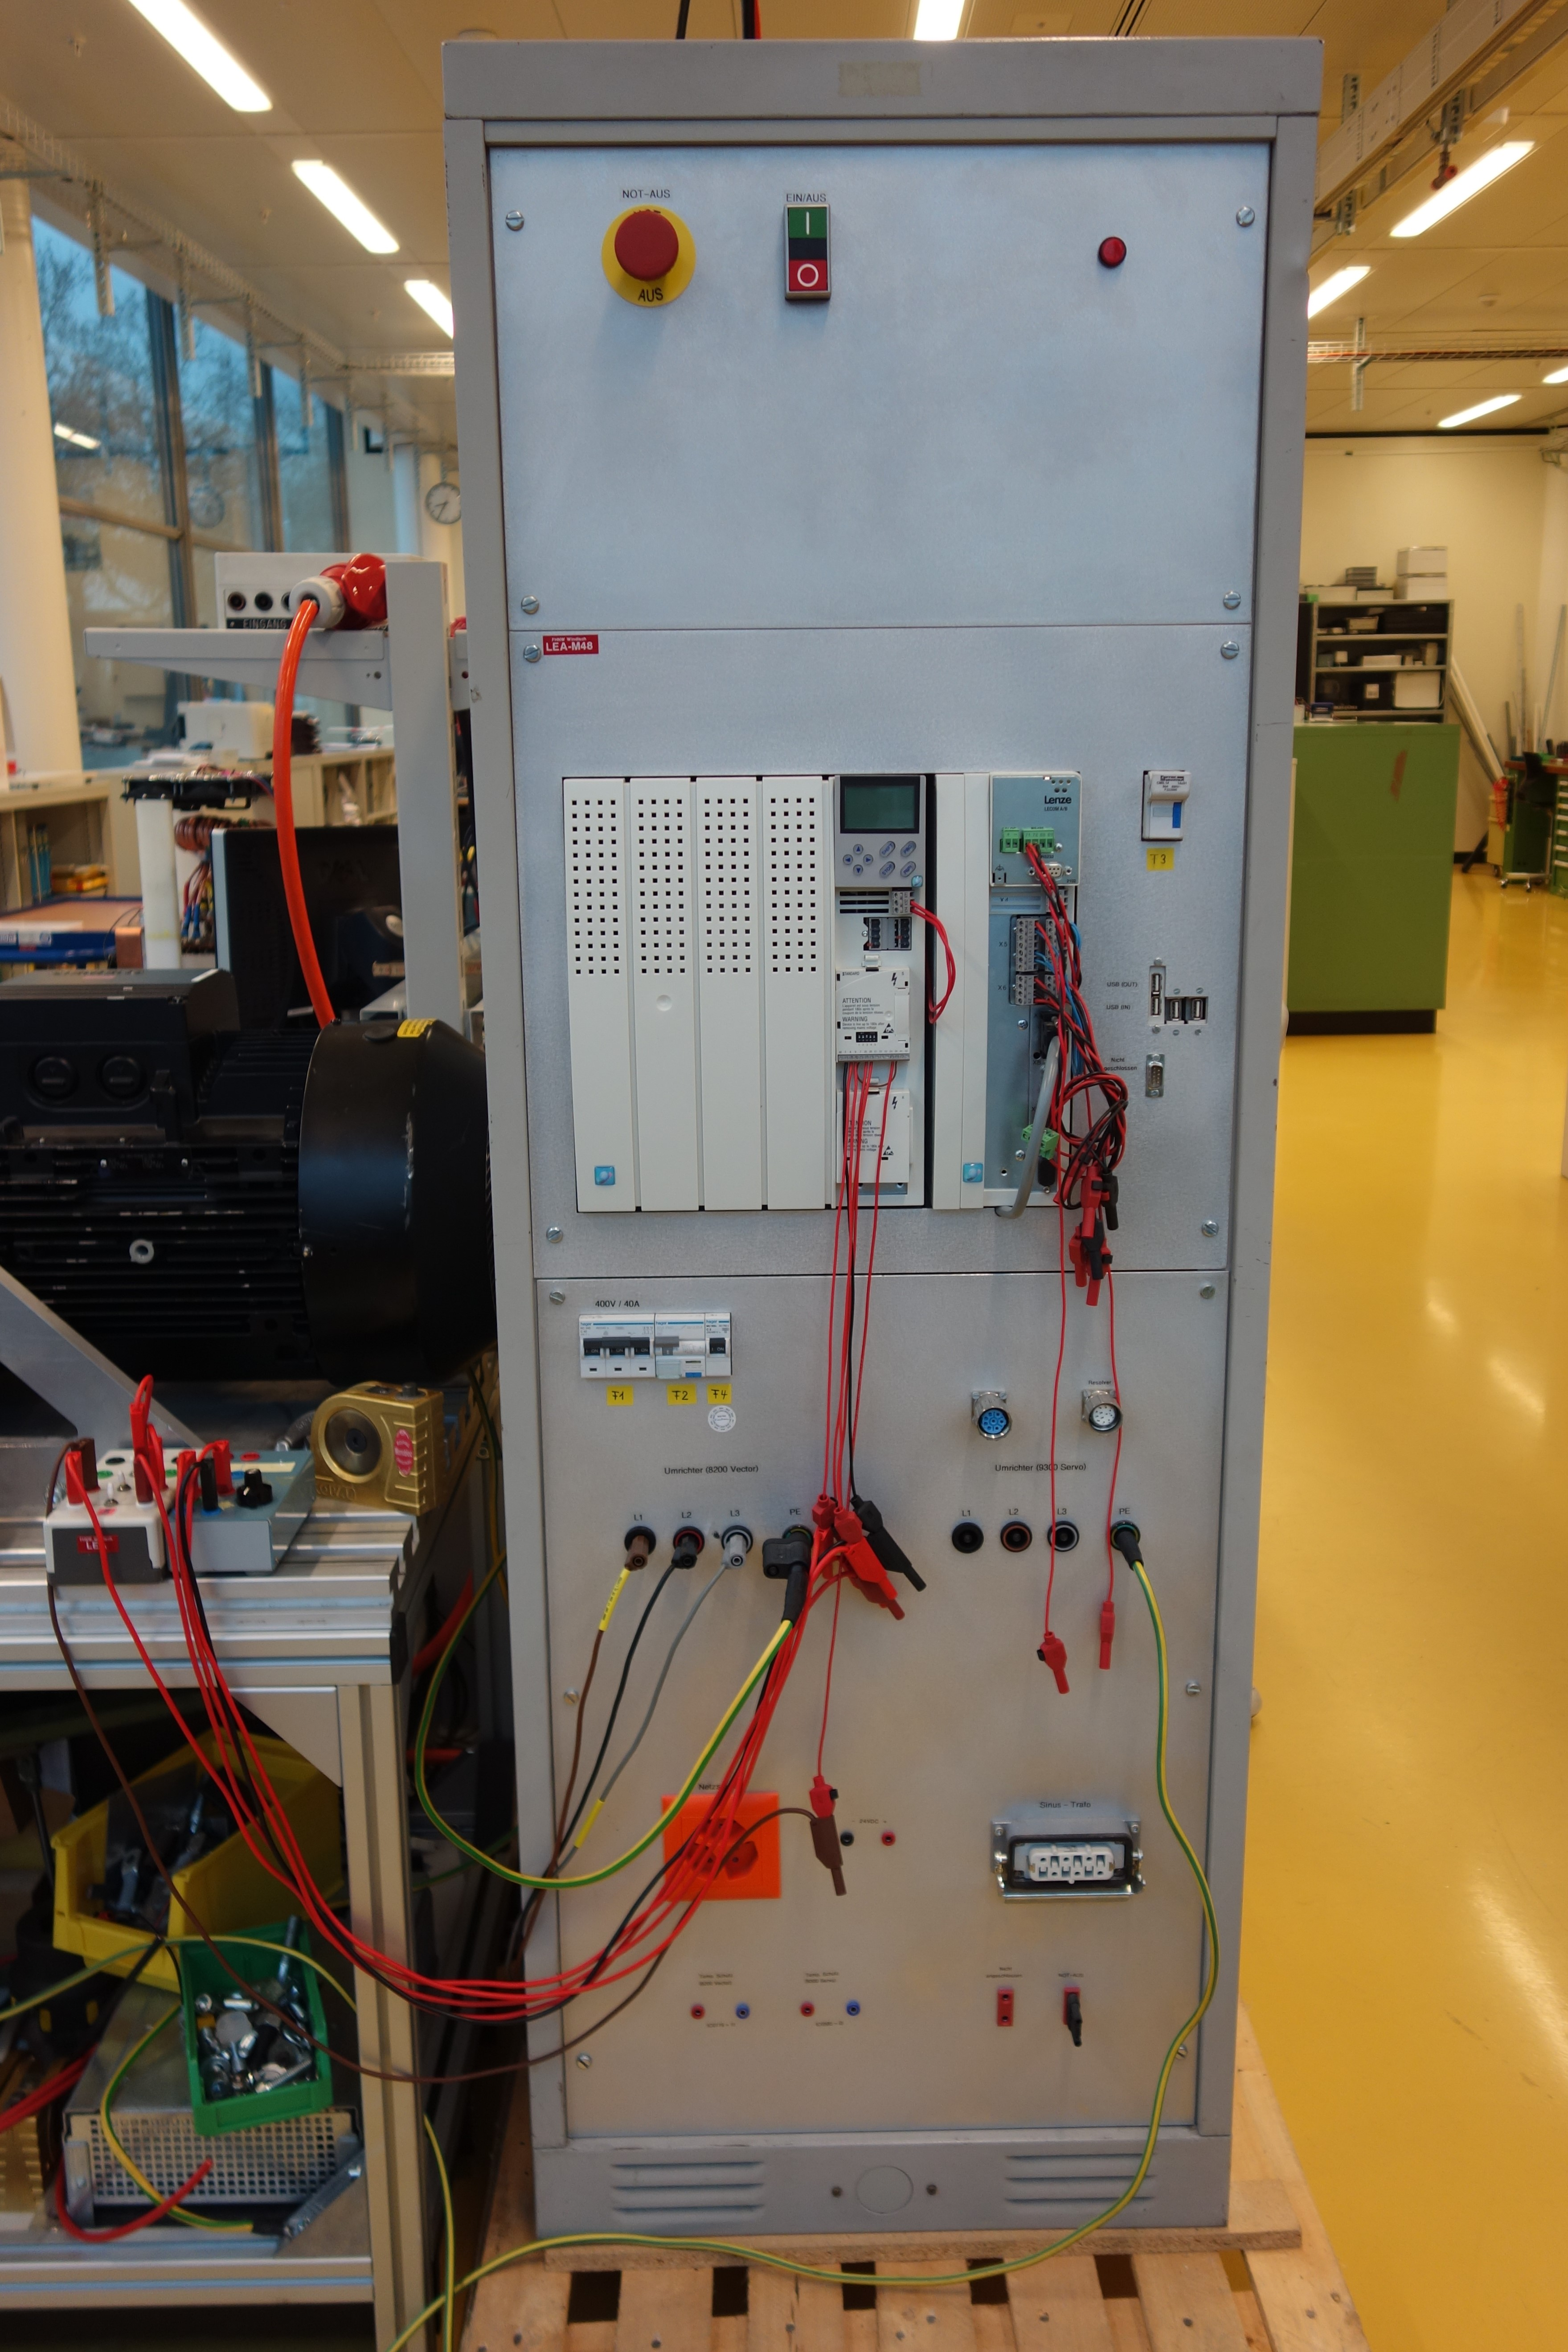
\includegraphics[height=100mm]{Versuchsaufbau/DSC00575.jpg}
		\caption[Frequenzumformer]{Frequenzumformer}
		\label{fig:Frequenzumformer}
	\end{minipage}
	\quad % Abstand zwischen Bilder
	\begin{minipage}[h]{.4\linewidth} % [b] => Ausrichtung an \caption
		\centering
		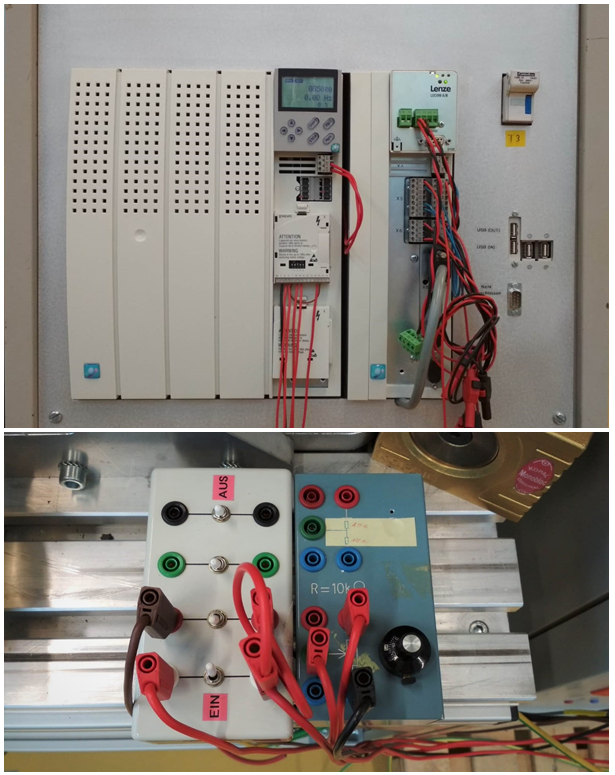
\includegraphics[width=\linewidth]{Versuchsaufbau/SteuerungRegelung.png}
		\caption[Ansteuerung und Regelung]{Ansteuerung und Regelung}
		\label{fig:AnsteuerungRegelung}
	\end{minipage}
\end{figure}

 Die Ansteuerung ist in Abbildung \ref{fig:AnsteuerungRegelung} ersichtlich, wobei die obere Grafik die Steuerungseinheit abbildet. In dieser können verschiedene Ansteuerungsverfahren (Frequenz oder Moment gesteuert) eingestellt werden. Ausserdem können diverse Parameter in der dazugehörigen Code-Tabelle verändert werden, wodurch die ASM optimal angesteuert werden kann. Durch die Veränderung der maximalen Frequenz kann indirekt die Maximaldrehzahl bestimmt werden. Die Frequenz wird durch eine Widerstandsänderung durch ein externes Potentiometer gegeben (Abbildung \ref{fig:AnsteuerungRegelung} unten rechts). Die externe Eingabe kann zudem die Steuerung aktivieren und die Drehrichtung ändern (unten links).

\newpage
\subsection{Drehmoment bei variabler Drehzahl}\label{subsec:DrehmomentDrehzahl}
Um zu beweisen, dass der Motor die erforderliche Leistung erbringt, wird das Drehmoment in Abhängigkeit der Drehzahl untersucht.
Die Bedingungen, mit welchen der Versuch durchgeführt wurde, können der Tabelle \ref{tab:Drehmoment/Drehzahl} entnommen werden.

\begin{table}[H]
\centering
\begin{tabular}{C{4cm} C{4cm} C{3cm}} 
\multicolumn{3}{c}{\textbf{Versuchsbedingungen}} \\
{Messgrösse}& {Bedingung} & {Wert}\\ \hline\hline 
Spannung (DC)   & nachgeregelt &   96 V     \\
Strom (DC)   & gemessen &   37.8-128 A     \\
Leistung (AC)   & gemessen &   1702-8870 W    \\
Drehzahl   & variiert &   614-2954 RPM    \\
Drehmoment-Sollwert   & nachgeregelt &   32 Nm    \\
Motor-Temperatur   & vernachlässigt &   -    \\
Controller-Temperatur   & vernachlässigt &   -    \\
\end{tabular}
\caption{Versuchsbedingungen Drehmoment/Drehzahl-Versuch}\label{tab:Drehmoment/Drehzahl}
\end{table}

Das Drehmoment an der Welle des BLDC-Motors wird mit der Formel \ref{eq:LeistungDrehmoment} in Abhängigkiet zur Leistung und der Drehzahl des Motors ermittelt. Die daraus ermittelte Kurve ist in der Abbildung \ref{fig:drehmoment/drehzahl} (blaue Kurve) ersichtlich. Da die asynchrone Maschine ebenfalls nicht ideal arbeitet und deswegen Verluste aufweist, wird bei dieser ein Wirkungsgrad von 90\% angenommen (rote Kurve).

\begin{equation}
\centering
P = M \cdot \omega = M \cdot 2 \cdot \pi\cdot f
\label{eq:LeistungDrehmoment}
\end{equation}
$P$\quad Leistung		\\
$M$\quad Drehmoment  \\
$\omega$\quad Winkelgeschwindigkeit\\
$f$\quad Frequenz	\\

\begin{figure}[H]
	\centering
	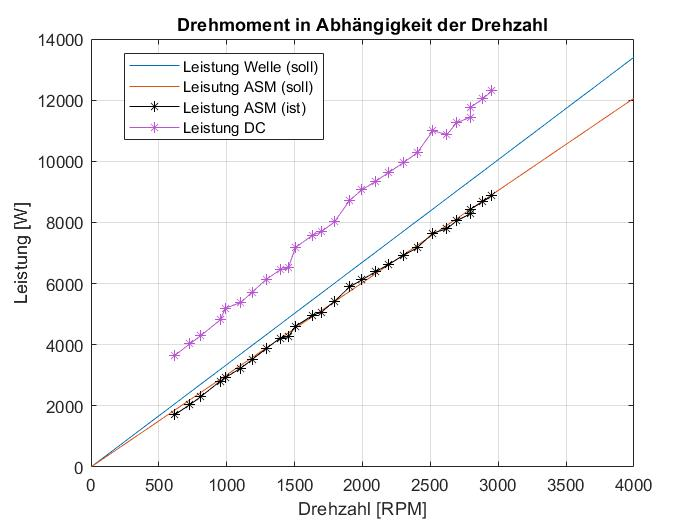
\includegraphics[width=1\linewidth]{drehmoment_drehzahl.jpg}
	\caption{Drehmoment in Abhängigkeit der Drehzahl}\label{fig:drehmoment/drehzahl}
\end{figure}

Bei diesem Versuch ist ersichtlich, dass es möglich ist, die erforderliche Leistung (schwarze Punkte) im Drehzahlbereich zwischen 600 und 3000 RPM (engl. revolutions per minute; \glqq Umdrehungen pro Minute\grqq) zu erreichen. Die aufgenommene Leistung auf der DC-Seite (violette Punkte) ist dabei proportional zur abgegebenen Leistung angestiegen und erreicht bei 3000 RPM einen Wert von über 12kW.

\newpage

In der Abbildung \ref{fig:drehmoment/StromSpannung} sind die Spannung, der Strom und die Sollwertvorgabe für die Ansteuerung während des Versuchs ersichtlich. Die Spannung ist auf $96V_{DC}$ nachgeregelt (blaue Punkte) worden, damit diese für den Versuch konstant bleibt. Der Strom (rote Punkte) und der Sollwert für die Ansteuerung (schwarze Punkte) wurden ebenfalls während des Versuchs dokumentiert.


\begin{figure}[H]
	\centering
	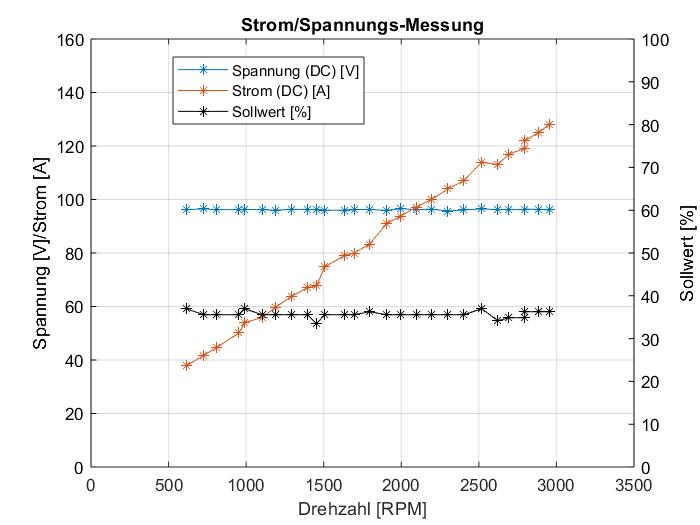
\includegraphics[width=1\linewidth]{drehmoment_StromSpannung.jpg}
	\caption{Spannung und Strom während des Drehmomentversuchs}\label{fig:drehmoment/StromSpannung}
\end{figure}

Der Strom kann mit guter Näherung als linear zur Drehzahl bei gleichbleibendem Drehmoment betrachtet werden. Dadurch ergibt sich bei 3800 RPM ein Strom von ca. 160A, was mit den Werten aus dem Datenblatt des Motors korreliert \cite{MotorData}. Diese maximale Leistung konnte mit diesem Versuchsaufbau jedoch nicht getestet werde, da dieser nur für 11kW ausgelegt ist (Kapitel \ref{subsec:Versuchsaufbau}).

Bei diesem Versuch ist ebenfalls ersichtlich, dass die Sollwertvorgabe über den Drehzahlbereich nur kleine Abweichungen aufweist und daher in guter Näherung als konstant betrachtet werden kann. Die Sollwertvorgabe wurde in Prozent des Minimums (1,2V) und des Maximums (4V) angegeben. Eine genauere Analyse des Sollwertvorgabe ist im Unterkapitel \ref{subsec:Steuerkennlinie} bei der Validierung der Steuerkennlinie ersichtlich.

\subsection{Leistungsabhängigkeit der Temperatur}\label{subsec:Leistung/Temperatur}
Da der BLDC-Motor eine sehr kleine Bauform für seine Leistung hat, unterliegt er grossen Temperaturschwankungen. Deshalb wird untersucht, wie sich die Temperatur bei konstantem Sollwert auf die Leistung auswirkt. Die Versuchsbedingungen können der Tabelle \ref{tab:Leistung/Temperatur} entnommen werden.


\begin{table}[H]
	\centering
	\begin{tabular}{C{4cm} C{4cm} C{3cm}} 
		\multicolumn{3}{c}{\textbf{Versuchsbedingungen}} \\
		{Messgrösse}& {Bedingung} & {Wert}\\ \hline\hline 
		Spannung (DC)   & nachgeregelt &   96 V     \\
		Strom (DC)   & gemessen &   106-112 A     \\
		Leistung (AC)   & gemessen &   7330-7820 W    \\
		Drehzahl   & konstant &   2500 RPM    \\
		Drehmoment-Sollwert   & konstant &   32 Nm    \\
		Motor-Temperatur   & gemessen &   30-100 °C    \\
		Controller-Temperatur   & vernachlässigt &   -    \\
	\end{tabular}
	\caption{Versuchsbedingungen Leistung/Temperatur-Versuch}\label{tab:Leistung/Temperatur}
\end{table}

Wie in der Abbildung \ref{fig:Leistung/Temperatur} ersichtlich ist, nimmt die Leistung bei zunehmender Temperatur ab. Die Leistung verringert sich bei einer Motor-Temperatur von 100°C (gegenüber 30°C) um ca. 6\%. Die Leistungsabnahme ist dabei in guter Näherung linear zur Temperatur.

\begin{figure}[H]
	\centering
	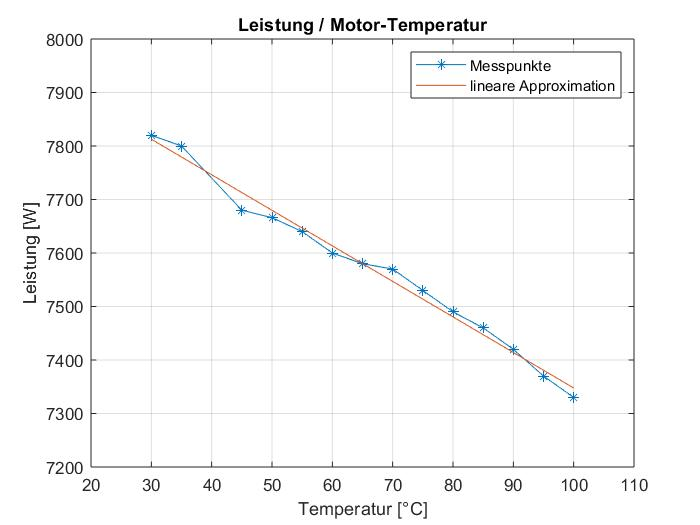
\includegraphics[width=0.9\linewidth]{LeistungTemperatur.jpg}
	\caption{Einfluss der Erwärmung auf die Leistung}\label{fig:Leistung/Temperatur}
\end{figure}

Wird in einem der nachfolgenden Versuche erwähnt, dass die Leistungs-Temperaturabhängigkeit berücksichtigt wurde, ist dies gleichbedeutend mit einer Temperaturskalierung aller Messwerte auf eine Temperatur von 70°C. Dies wird durch Einkalkulierung der in diesem Versuch ermittelte lineare Approximation erreicht, wodurch jeder einzelne Messwert schlussendlich dasselbe Temperaturniveau besitzt und somit die Messung temperaturunabhängig ist.
\subsection{Steuerkennlinie}\label{subsec:Steuerkennlinie}
Die Steuerkennlinie beschreibt die Funktion zwischen dem Input (entspricht einem Regelsignal zwischen 1.2-4V) und dem Drehmoment-Sollwert. Bei diesen Messungen geht es darum, diese Funktion zu bestimmen, um später das angelegte Moment am Motor ohne direkte Kraftmessung regeln zu können. Die Versuchsbedingungen sind in nachfolgender Tabelle \ref{tab:Steuerkennlinie} aufgeführt:

\begin{table}[H]
	\centering
	\begin{tabular}{C{4cm} C{4cm} C{3cm}} 
		\multicolumn{3}{c}{\textbf{Versuchsbedingungen}} \\
		{Messgrösse}& {Bedingung} & {Wert}\\ \hline\hline 
		Spannung (DC)   & nachgeregelt &   96 V     \\
		Strom (DC)   & gemessen &   1.6-107 A     \\
		Leistung (AC)   & gemessen &   0-5666 W    \\
		Drehzahl   & konstant &   1200 RPM    \\
		Drehmoment-Sollwert   & variiert &   0-50 Nm    \\
		Motor-Temperatur   & gemessen &   40-100 °C    \\
		Controller-Temperatur   & vernachlässigt &   -    \\
	\end{tabular}
	\caption{Versuchsbedingungen Steuerkennlinie}\label{tab:Steuerkennlinie}
\end{table}

Wie in der Abbildung \ref{fig:Leistung/Steuerkennlinie} ersichtlich ist, lässt sich das Verhältnis zwischen Drehmoment und Regelsignal mit einer quadratischen Funktion beschreiben. Bei diesem Versuch wird die Leistungs-Temperaturabhängigkeit berücksichtigt, wie sie im Unterkapitel \ref{subsec:Leistung/Temperatur} erklärt wurde.

\begin{figure}[H]
	\centering
	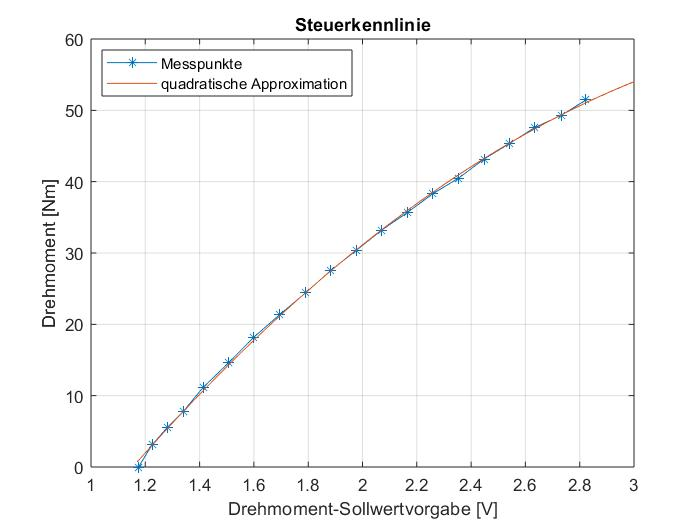
\includegraphics[width=0.9\linewidth]{Steuerkennlinie.jpg}
	\caption{Steuerkennlinie der Ansteuerung}\label{fig:Leistung/Steuerkennlinie}
\end{figure}

Da der Motor bei diesem Versuch an die thermische Grenze kam und für die geplante Anwendung keine höhere Drehmomente erforderlich sind, wird die Messung nur bis 2.8V durchgeführt. Das Maximum des Drehmoment-Sollwertes liegt jedoch bei 4V.
\subsection{Leistungsverhalten bei Spannungsabfall}\label{subsec:LeistungSpannungabfall}
Bei diesem Versuch wird das Verhalten des Controllers bei einem Spannungsabfall untersucht. Dabei wurde sowohl die Leistung der ASM (Abbildung \ref{fig:Spannungsabfall} rechts) als auch der Strom des Controllers (Abbildung \ref{fig:Spannungsabfall} links) in Abhängigkeit zur Spannung des Controllers gemessen. Der Drehmoment-Sollwert wurde während des gesamten Versuchs konstant auf dem Nennmoment gehalten. Die Versuchsbedingungen können der Tabelle \ref{tab:Spannungsabfall} entnommen werden.

\begin{table}[H]
	\centering
	\begin{tabular}{C{4cm} C{4cm} C{3cm}} 
		\multicolumn{3}{c}{\textbf{Versuchsbedingungen}} \\
		{Messgrösse}& {Bedingung} & {Wert}\\ \hline\hline 
		Spannung (DC)   & variiert &   72-103 V     \\
		Strom (DC)   & gemessen &   68.7-124 A     \\
		Leistung (AC)   & gemessen &   4420-6420 W    \\
		Drehzahl   & variiert &   1500/2000 RPM    \\
		Drehmoment-Sollwert   & konstant &   32 Nm    \\
		Motor-Temperatur   & gemessen &   30-90 °C    \\
		Controller-Temperatur   & vernachlässigt &   -    \\
	\end{tabular}
	\caption{Versuchsbedingungen Spannungsabfall}\label{tab:Spannungsabfall}
\end{table}


Auf der Abbildung \ref{fig:Spannungsabfall} sind die Messwerte des Versuchs dargestellt. Zuerst wurde der Versuch mit 2000 RPM (blaue Punkte) und danach nochmals mit 1500 RPM (rote Punkte) durchgeführt. Wird die Leistungs-Temperaturabhängigkeit berücksichtigt (schwarze und rosa Punkte), dann ist ersichtlich, dass die Leistung nicht von der Spannung, sondern lediglich von der Temperatur abhängig ist.

\begin{figure}[H]
	\centering
	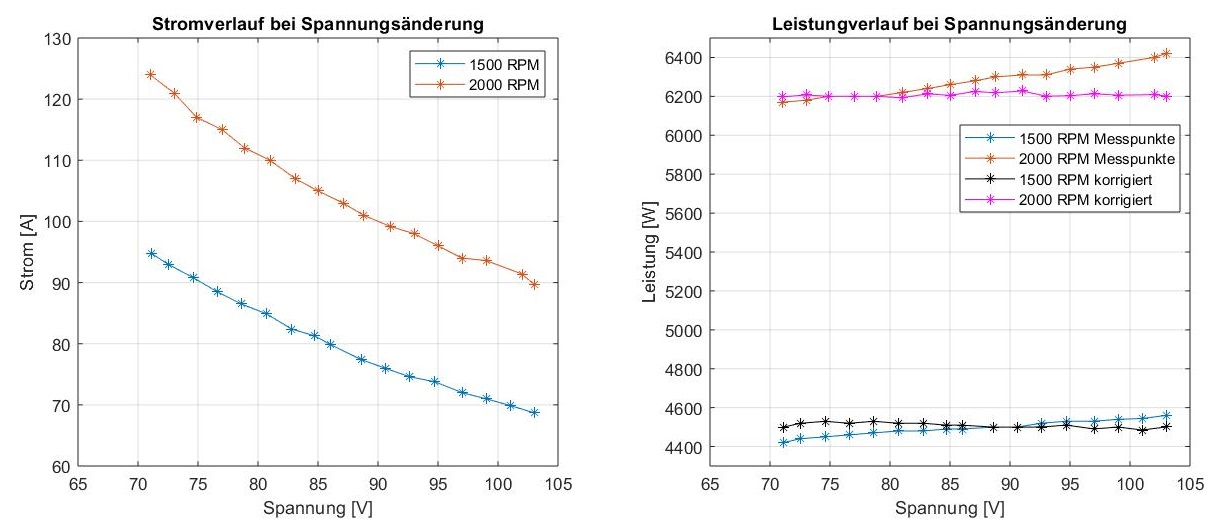
\includegraphics[width=1\linewidth]{Spannungsversuch.jpg}
	\caption{Leistungs- und Stromverlauf bei Spannungsabfall}\label{fig:Spannungsabfall}
\end{figure}

\subsection{Temperatur}\label{subsec:Temperatur}
Um einen Einblick in das Temperaturverhalten des Motors zu erlangen, wurde in diesem Versuch die Erwärmung in Abhängigkeit der Drehzahl bei konstantem Moment gemessen. Die Messung erfolgte bei einer Drehzahl von 1550 RPM und bei 2550 RPM, und einem jeweiligen Drehmoment von 32Nm. Die Starttemperatur des Motors lag jeweils bei ca. 60°C und wurde solang betrieben, bis er eine Betriebstemperatur von 100°C erreicht hatte.


\begin{figure}[H]
	\centering
	\includegraphics[width=0.8\linewidth]{Temperatur.jpg}
	\caption{Erwärmung}\label{fig:Temperatur}
\end{figure}


Da die Leistung sowohl vom Drehmoment als auch von der Drehzahl abhängig ist, wurde beim Versuch bei 2550RPM eine höhere Leistung und somit auch ein grösseren Strom erzielt. Aus diesem Grund ist die Erwärmung des Motors bei höheren Drehzahlen dementsprechend grösser. Anhand der beiden Versuchen gehen wir davon aus, dass der BLDC-Motor ca. 5 Minuten unter Vollast betrieben werden kann, bis er die 100°C erreicht. Es gilt zu beachten, dass der Motor eine Betriebstemperatur von 110°C zulässt, wodurch eine Reserve von 10°C gegeben ist.
\subsection{Maximale Leistung bei variabler Spannung}\label{subsec:LeistungSpannungsabfall}
In diesem Versuch wird die maximale Leistung bei einem Spannungsabfall untersucht. Da die asynchrone Maschine nicht für 3800 RPM ausgelegt ist, wurde dieser Versuch bei einer konstanten Drehzahl von 3600 RPM gemessen. Wie im vorhergehenden Versuch, wurde das Drehmoment aufs Maximum eingestellt, während die Spannung langsam erhöht wurde.


\begin{figure}[H]
	\centering
	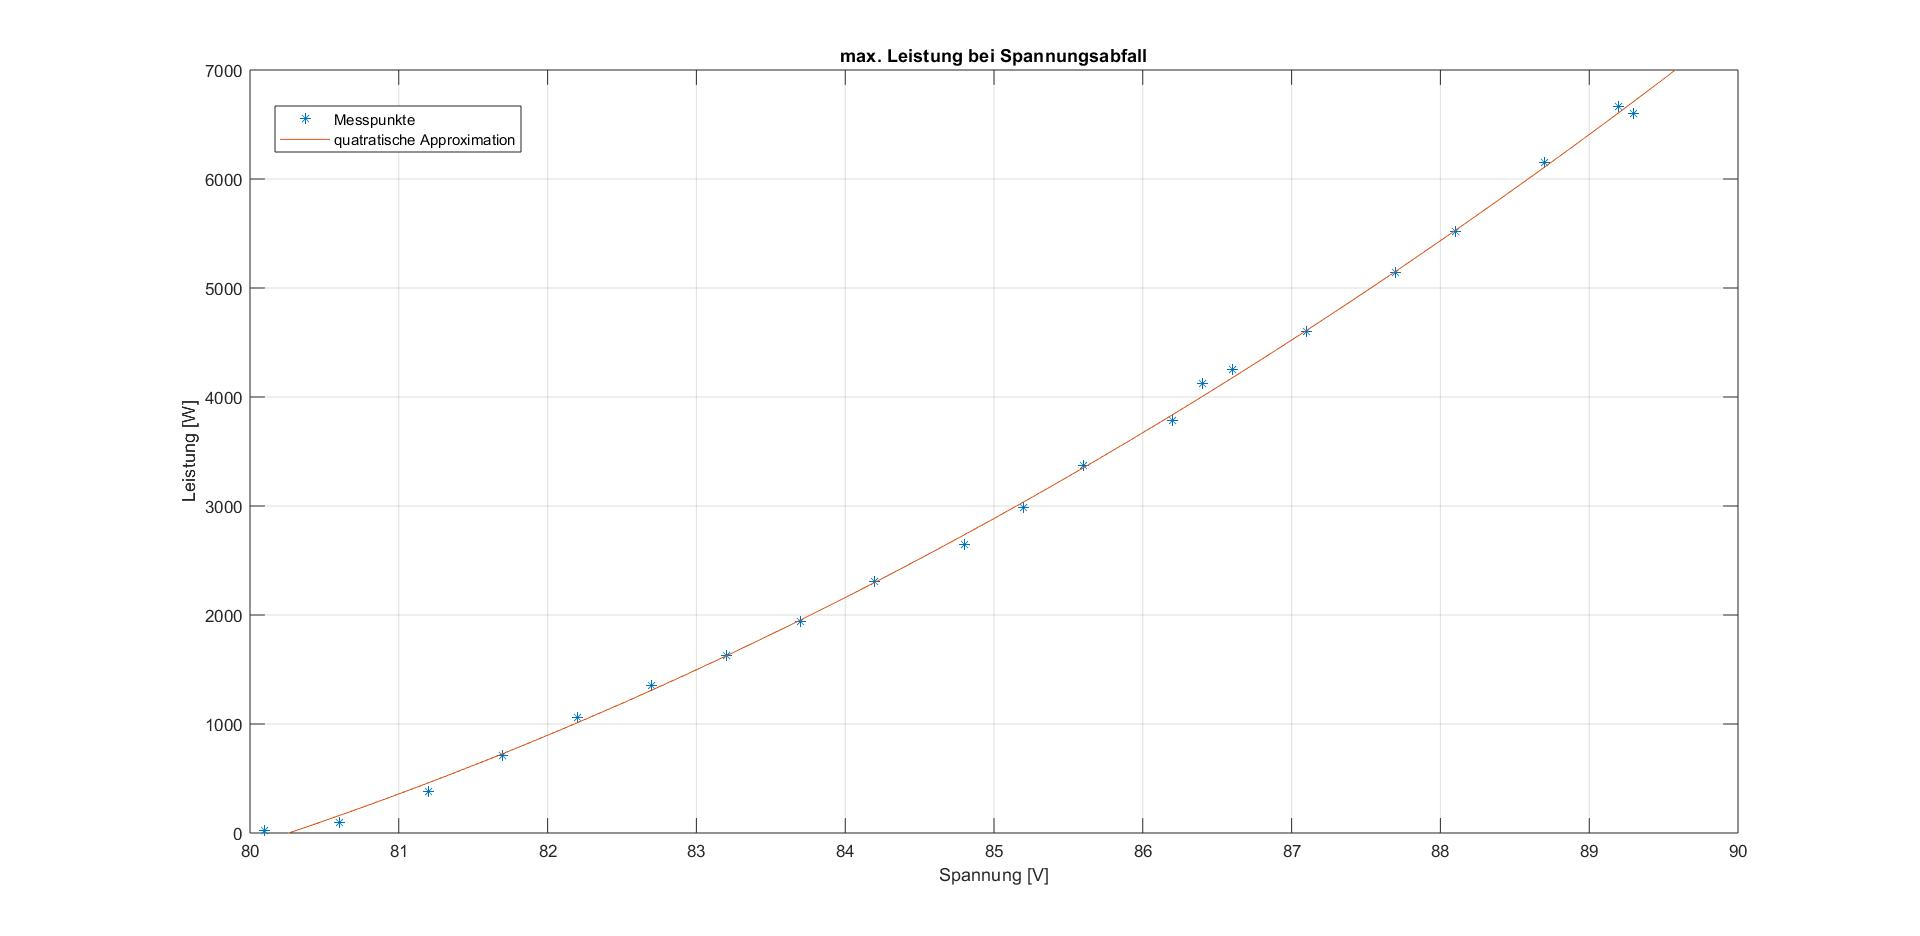
\includegraphics[width=0.8\linewidth]{maxLeistung.jpg}
	\caption{Maximale Leistung}\label{fig:maxLeistung}
\end{figure}

Unter der Annahme, dass zwischen der maximalen Leistung und der Spannung ein quadratischer Zusammenhang besteht (rote Approximation), ist anzunehmen, dass die maximale Leistung bei 3600 RPM und Nennspannung (96V) bei 15kW liegt. Hierbei ist jedoch anzumerken, dass die effektive Leistung an der Welle des BLDC-Motors ca. 10\% höher ist, da diese auf der elektrischen Seite der asynchronen Maschine gemessen wurde.
 
\subsection{Maximale Drehzahl bei variabler Spannung}\label{subsec:DrehzahlSpanungsabfall}
In diesem Versuch wird das Verhalten des Motors bei Unterspannung untersucht. Dabei wird der Sollwert für das Drehmoment auf dem Maximum gehalten, während der Motor im Leerlauf dreht. Die Spannung wird dabei langsam erhöht.

\begin{table}[H]
	\centering
	\begin{tabular}{C{4cm} C{4cm} C{3cm}} 
		\multicolumn{3}{c}{\textbf{Versuchsbedingungen}} \\
		{Messgrösse}& {Bedingung} & {Wert}\\ \hline\hline 
		Spannung (DC)   & variiert &   64.7-90.7 V     \\
		Strom (DC)   & gemessen &   9.33-13.1 A     \\
		Leistung (AC)   & vernachlässigt &   -    \\
		Drehzahl   & gemessen &   3600 RPM    \\
		Drehmoment-Sollwert   & konstant &   max.    \\
		Motor-Temperatur   & vernachlässigt &   -    \\
		Controller-Temperatur   & vernachlässigt &   -    \\
	\end{tabular}
	\caption{Versuchsbedingungen max. Drehzahl}\label{tab:maxDrehzahl}
\end{table}

Damit der Motor nicht durch zu hohe Drehzahlen beschädigt wird, kann beim Controller eine Drehzahlobergrenze eingestellt werden. Diese ist für diesen Versuch auf 3800 RPM begrenzt, weil die asynchrone Maschine keine höheren Drehzahlen zulässt. Die maximale Drehzahl ist in nachfolgender Abbildung \ref{fig:maxDrehzahl} graphisch dargestellt.

\begin{figure}[H]
	\centering
	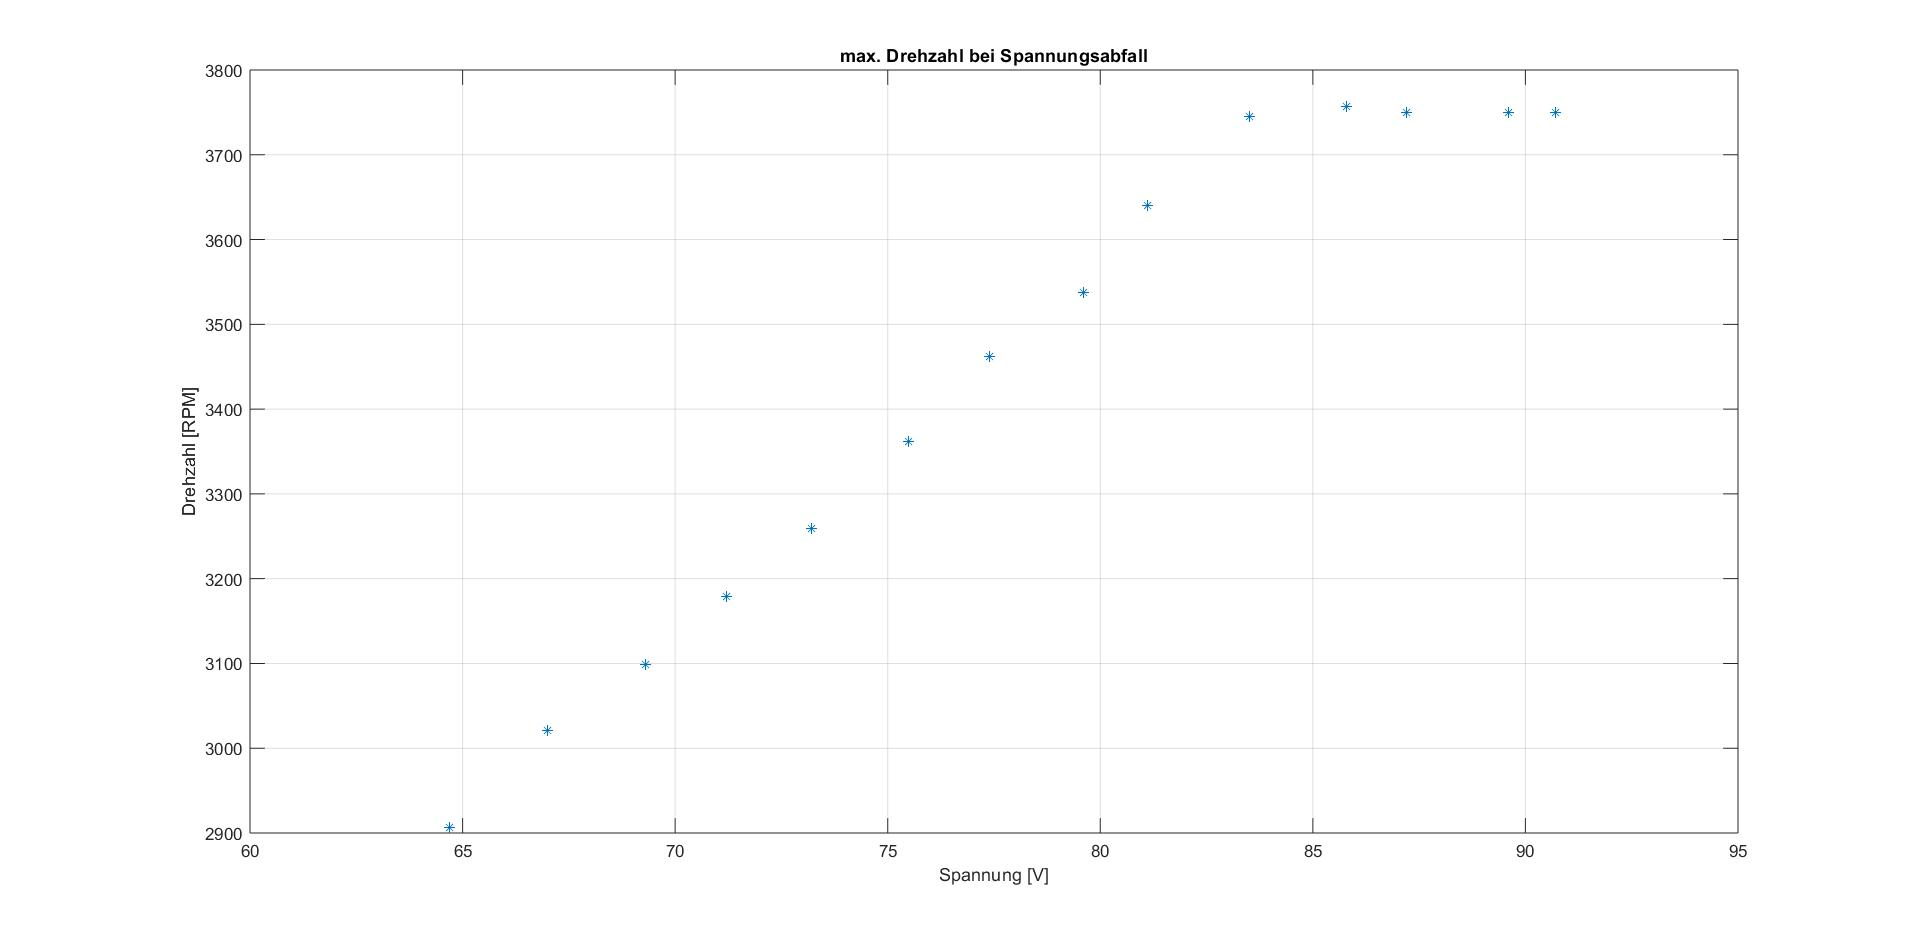
\includegraphics[width=0.8\linewidth]{maxDrehzahl.jpg}
	\caption{Maximale Drehzahl im Leerlauf}\label{fig:maxDrehzahl}
\end{figure}


Bei diesem Versuch hat sich gezeigt, dass die DC-Spannung mindestens 84V betragen muss, damit der BLDC-Motor in Feldschwächung kommt und somit eine Drehzahl von 3800 RPM erreichen kann. Weiter ist ersichtlich, dass die Leerlaufdrehzahl ca. 45 RPM pro Volt sinkt.


\section{Offene Arbeiten}
Um die Arbeit erfolgreich und möglichst speditiv fortzuführen, werden in diesem Kapitel die noch offenen Arbeiten und die weiteren Schritte, welche verfolgt werden erläutert.

Nach diversen erfolgreichen Tests am Motor konnten wir praktisch alle Anforderungen (Anhang \ref{appsec:Anforderungen}) an den Einzugswindenbetrieb erledigen. Da das Produkt aber sowohl einen Einzugs- als auch einen Abrollwindenbetrieb garantieren soll, muss in einem weiteren Schritt der Motor im Betrieb als Generator getestet werden. Damit dies erfolgreich erledigt werden kann, muss eine Bremsschaltung aufgebaut werden, welche die rekuperierte Energie des BLDC-Motors in Wärme umwandeln kann. Beim Abrollbetrieb können Leistungen von bis zu 10kW entstehen. Diese Leistung wird primär benutzt um die Batterien zu laden, sobald diese jedoch geladen sind, muss diese Energie verheizt werden. Diese Heizwiderstände und die dazugehörige Schaltung muss dafür dimensioniert werden.

Die Auswahl der Batterie ist aus diesem Grund nicht nur für die Energieversorgung des Motors von grosser Bedeutung, sondern auch für den Abrollbetrieb. Aus diesem Grund ist auch diese Anschaffung ein weiterer Bestandteil, welcher als Nächstes ins Auge gefasst werden muss. Mit der Anschaffung von Batterien ist das ganze Thema der Energieversorgung jedoch noch nicht erledigt. Es ist ein Ladegerät notwendig, sofern die Winde nur als Einzugswinde betrieben wird. Zudem ist auch eine Batterieüberwachung notwendig, welche die Batterie gegen Über-, und Tiefenentladung schützt und vorzeitig warnt. Wie diese Warnung erreicht wird, fällt in die Ausarbeitung der Bedieneinheit, welche ebenfalls ausgearbeitet werden muss. Die Ansteuerung des Motors mit den unterschiedlichen Start Abläufen, die Bedienung des Not-Aus, eine mögliche visuelle Anzeige über aktuelle Parameter und die Positionierung stehen zudem im Fokus.

Zum Schutz vor Berührung, werden alle elektronischen Komponenten (wie Controller, Chopper-Schaltung, usw.) in einen Schaltschrank eingebaut, welcher ebenfalls eine Sicherung über das Gesamtsystem enthält. Die damit verbundene Übersichtlichkeit ist zudem wartungsfreundlich und ermöglicht rasche Anpassungen. Weiter ist gemäss DHV-Reglement eine Rundumleuchte zur Betriebssignalisation erforderlich.\\
Zum Schluss stehen noch zahlreiche Tests bevor. Die Anlage wird zuerst im und ausserhalb des Labors unter idealen Bedingungen getestet, bevor der erste Gleitschirmflieger in einem Feldversuch hochgezogen wird.
\section{Schlusswort}\label{sec:Schlusswort}

In dieser Arbeit wurde versucht, alle elektrisch betriebenen Bestandteile einer Schleppwinde in Abrollwinden- und Einzugswindenbetrieb zu definieren und mittels Laborversuchen auszutesten. Dabei galt es alle Anforderungen an eine Schleppwinde (gemäss dem deutschen Hängegleiterverbande) zu beachten und dementsprechend alle Bestandteile nach den geforderten Normen auszulegen.

Die Ergebnisse der Labortests zeigen, dass der Motor alle Anforderungen im Einzugswindenbetrieb erfüllt. Die Ansteuerung des Motors erfolgt mittels eines Controllers und verläuft ebenfalls optimal. Hierbei kann eine maximale Drehzahl vorgegeben werden, welche vom Motor bei Normalbetrieb nicht überschritten werden kann. Dadurch lässt garantieren, dass eine Geschwindigkeit des Seileinzugs von 10m/s nicht überschritten wird. Auch bei Lastabwurf, regelt der Controller extrem schnell und reduziert die Geschwindigkeit des Motors auf die gewünschte Drehzahl herunter. Weiter können Drehmomentsollwerte über den Controller sehr einfach vorgegeben und vom Motor angefahren werden. Weiter kann trotz Leistungsänderungen während dem Betrieb keine Welligkeit festgestellt werden. Erfreulich ist auch das Leistungsverhalten bei Änderungen der Temperatur mit einer Abweichung von lediglich 6\% über den ganzen Temperaturbereich (30°C zu 100°C). Auch der Betrieb in Feldschwächung funktioniert einwandfrei, wobei beachtet werden muss, dass diese von der Spannungsversorgung abhängig ist. Unterschreitet die Spannungsversorgung 84V, so kann die Drehzahl von 3800U/min (entspricht Drehzahl im Nennarbeitspunkt) auch im Leerlauf nicht mehr erreicht werden. Wird der Motor unterhalb der Nennspannung (96V) betrieben, kann er das Nennmoment bei hohen Drehzahlen nicht mehr erbringen, dadurch ergibt sich eine Leistungsgrenze, welche von der Versorgungsspannung abhängig ist. Damit diese so klein wie möglich ist, darf die Energieversorgung auch unter starker Belastung keinen Markanten Spannungseinbruch aufweisen.

Leider konnte in diesem Projekt mangels Zeit der Abrollwindenbetrieb nicht ausgearbeitet werden. Aus diesem Grund soll als nächstes genau dieser ausgelegt und getestet werden. Dafür sind sowohl Batterien als auch Heizwiderstände und die dazugehörige Elektronik notwendig. Mit diesen Komponenten wird der Versuchsaufbau erweitert, damit der Motor sowohl im Einzugswindenbetrieb als auch Abrollwindenbetrieb betrieben und validiert werden kann. Während der mechanische Teil konstruiert und aufgebaut wird, wird das Bedieninterface und die übrigen Bauteile entwickelt, damit am Anfang des nächsten Sommers die ersten Feldversuche möglich sind.


\section{Bibliographien}
\printbibliography


%%---BIBLIOGRAPHY------------------------------------------------------------------------
{\sloppypar
%\printbibliography[heading=bibintoc]
%\label{sec:lit}
\selectlanguage{english}				%ngerman or english
}

%%---APPENDIX----------------------------------------------------------------------------
\begin{appendix} %Anhang


\includepdf[pages={1-2},nup=1x2,landscape=true,scale=0.85,offset=10 -40,pagecommand={\section{Eingefügtes Dokument; zwei Seiten auf einer}\label{app:Aufgabenstellung}\thispagestyle{myheadings}}]{appendix/aufgabenstellung.pdf} \newpage
%%Bei mehrseitigen Dokumenten die folgenden Seiten ohne Überschrift:
%
\includepdf[pages={3-6},nup=1x2,landscape=true,scale=0.85,offset=10 -40,pagecommand={\thispagestyle{myheadings}}]{appendix/aufgabenstellung.pdf} \newpage

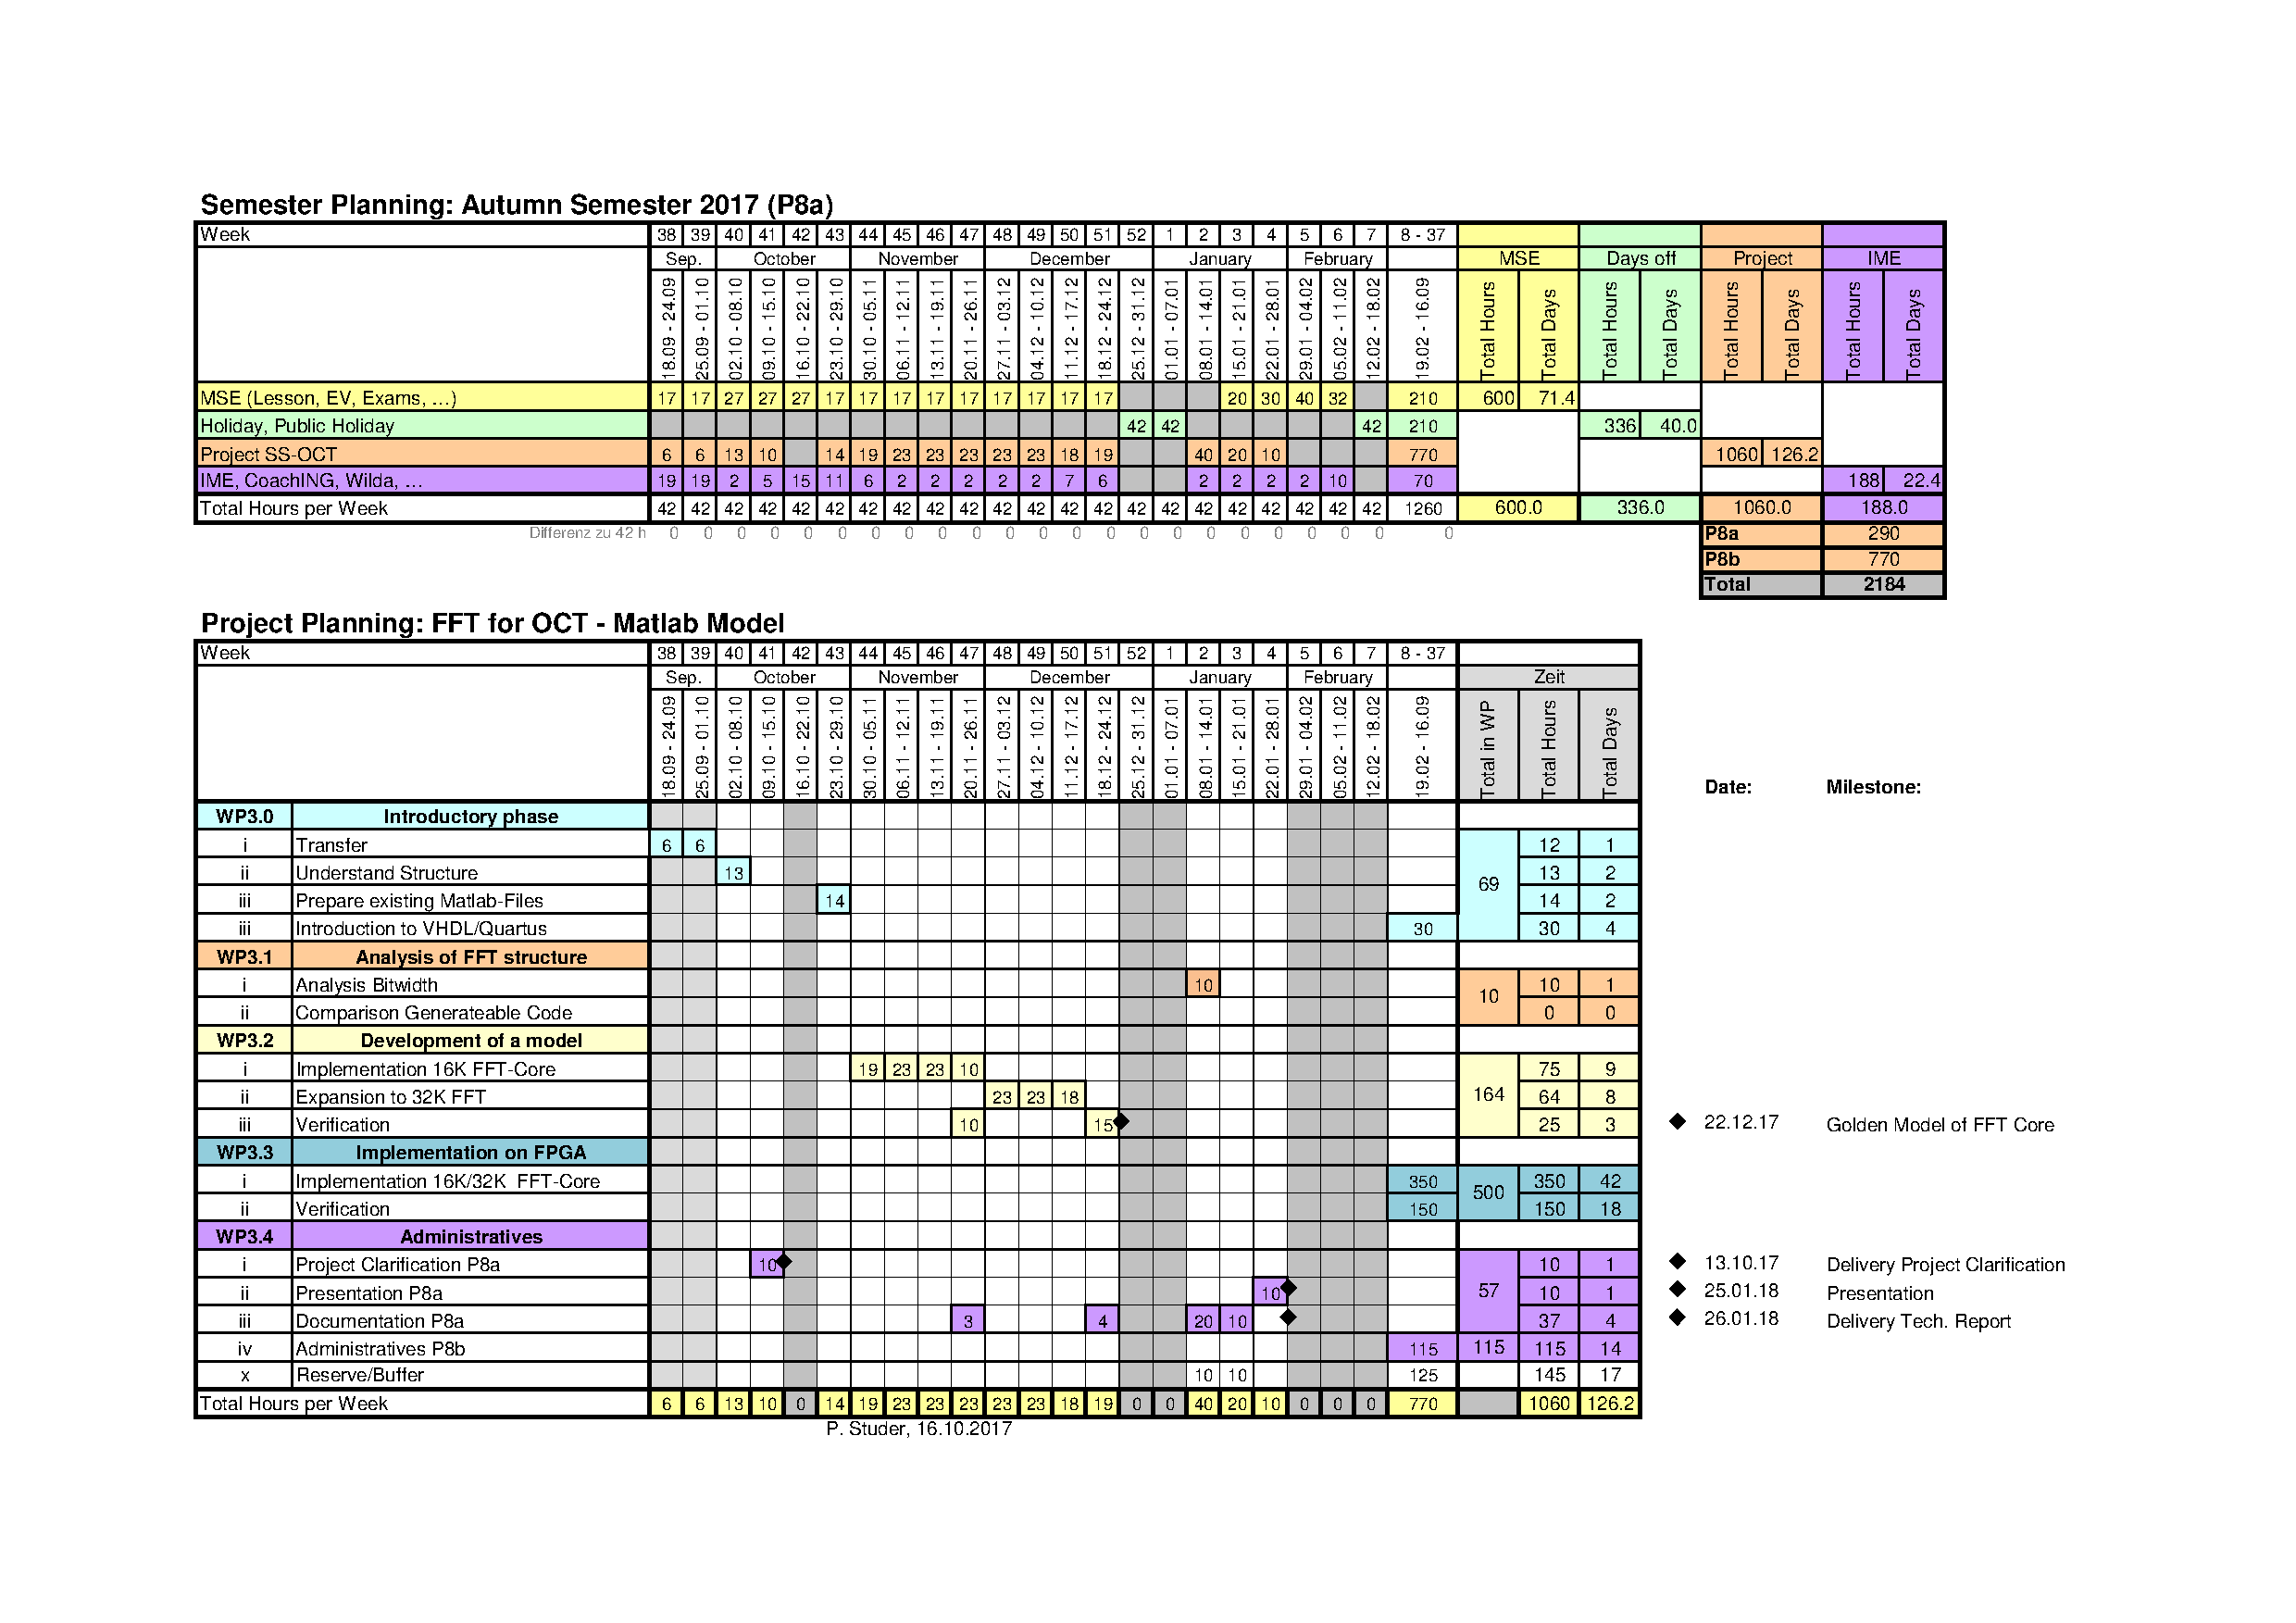
\includepdf[pages={1},nup=1x1,landscape=true,scale=0.85,offset=10 -40,pagecommand={\section{Eingefügte PDF-Tabelle}\label{app:Timetable}\thispagestyle{myheadings}}]{appendix/timeline_example.pdf} \newpage
%%Bei mehrseitigen Dokumenten die folgenden Seiten ohne Überschrift:
%\includepdf[pages={2-5},nup=1x1,landscape=true,scale=0.85,offset=0 -20,pagecommand={\thispagestyle{myheadings}}]{appendix/timeline_example.pdf} \newpage

\section{MATLAB-Code Snippets}
\lstinputlisting{appendix/code/matlab.m}


\end{appendix}


%%---NOTES for DEBUG---------------------------------------------------------------------
\ifdraft{%Do this only if mode=draft
%%requires \usepackage{todconotes})
\newpage
\listoftodos[\section{Todo-Notes}]
\clearpage
}
{%Do this only if mode=final
}
\end{document}

